%  A simple AAU report template.
%  2015-05-08 v. 1.2.0
%  Copyright 2010-2015 by Jesper Kjær Nielsen <jkn@es.aau.dk>
%
%  This is free software: you can redistribute it and/or modify
%  it under the terms of the GNU General Public License as published by
%  the Free Software Foundation, either version 3 of the License, or
%  (at your option) any later version.
%
%  This is distributed in the hope that it will be useful,
%  but WITHOUT ANY WARRANTY; without even the implied warranty of
%  MERCHANTABILITY or FITNESS FOR A PARTICULAR PURPOSE.  See the
%  GNU General Public License for more details.
%
%  You can find the GNU General Public License at <http://www.gnu.org/licenses/>.
%
%% Uncomment these for your final PDF to reduce size (slows down compilation)
\documentclass[11pt,twoside,a4paper]{report}
%%%%%%%%%%%%%%%%%%%%%%%%%%%%%%%%%%%%%%%%%%%%%%%%
% Language, Encoding and Fonts
% http://en.wikibooks.org/wiki/LaTeX/Internationalization
%%%%%%%%%%%%%%%%%%%%%%%%%%%%%%%%%%%%%%%%%%%%%%%%
% Select encoding of your inputs. Depends on
% your operating system and its default input
% encoding. Typically, you should use
%   Linux  : utf8 (most modern Linux distributions)
%            latin1 
%   Windows: ansinew
%            latin1 (works in most cases)
%   Mac    : applemac
% Notice that you can manually change the input
% encoding of your files by selecting "save as"
% an select the desired input encoding. 
\usepackage[utf8]{inputenc}
% Make latex understand and use the typographic
% rules of the language used in the document.
\usepackage[danish,english]{babel}
% Use the palatino font
\usepackage[sc]{mathpazo}
\linespread{1.05}         % Palatino needs more leading (space between lines)
\usepackage{parskip}

% Choose the font encoding
\usepackage[T1]{fontenc}

%%%%%%%%%%%%%%%%%%%%%%%%%%%%%%%%%%%%%%%%%%%%%%%%
% Graphics and Tables
% http://en.wikibooks.org/wiki/LaTeX/Importing_Graphics
% http://en.wikibooks.org/wiki/LaTeX/Tables
% http://en.wikibooks.org/wiki/LaTeX/Colors
\usepackage{multirow}
%%%%%%%%%%%%%%%%%%%%%%%%%%%%%%%%%%%%%%%%%%%%%%%%
% load a colour package
\usepackage{xcolor}
\definecolor{aaublue}{RGB}{33,26,82}% dark blue
% The standard graphics inclusion package
\usepackage{graphicx,wrapfig,lipsum}

\usepackage{subcaption}
% Set up how figure and table captions are displayed
\usepackage{caption}
\captionsetup{%
  font=footnotesize,% set font size to footnotesize
  labelfont=bf % bold label (e.g., Figure 3.2) font
}
% Make the standard latex tables look so much better
\usepackage{array,booktabs}
% Enable the use of frames around, e.g., theorems
% The framed package is used in the example environment
\usepackage{framed}

% Adds support for full page background picture
\usepackage[contents={},color=gray]{background}
%\usepackage[contents=draft,color=gray]{background}

%%%%%%%%%%%%%%%%%%%%%%%%%%%%%%%%%%%%%%%%%%%%%%%%
% Mathematics
% http://en.wikibooks.org/wiki/LaTeX/Mathematics
%%%%%%%%%%%%%%%%%%%%%%%%%%%%%%%%%%%%%%%%%%%%%%%%
% Defines new environments such as equation,
% align and split 
\usepackage{amsmath}
% Adds new math symbols
\usepackage{amssymb}
% Include SI units
\usepackage{siunitx}
\usepackage{algpseudocode}
\usepackage{algorithm}

% Setup subfigures
\usepackage{caption}
\usepackage{subcaption}

% Use theorems in your document
% The ntheorem package is also used for the example environment
% When using thmmarks, amsmath must be an option as well. Otherwise \eqref doesn't work anymore.
\usepackage[framed,amsmath,thmmarks]{ntheorem}

%%%%%%%%%%%%%%%%%%%%%%%%%%%%%%%%%%%%%%%%%%%%%%%%
% Page Layout
% http://en.wikibooks.org/wiki/LaTeX/Page_Layout
%%%%%%%%%%%%%%%%%%%%%%%%%%%%%%%%%%%%%%%%%%%%%%%%
% Change margins, papersize, etc of the document
\usepackage[
  inner=28mm,% left margin on an odd page
  outer=28mm,% right margin on an odd page
  ]{geometry}
% Modify how \chapter, \section, etc. look
% The titlesec package is very configureable
\usepackage{titlesec}
\usepackage{lipsum}
\titleformat{\chapter}[display]{\normalfont\huge\bfseries}{\chaptertitlename\ \thechapter}{20pt}{\Huge}
\titleformat*{\section}{\normalfont\Large\bfseries}
\titleformat*{\subsection}{\normalfont\large\bfseries}
\titleformat*{\subsubsection}{\normalfont\normalsize\bfseries}
%\titleformat*{\paragraph}{\normalfont\normalsize\bfseries}
%\titleformat*{\subparagraph}{\normalfont\normalsize\bfseries}

% Clear empty pages between chapters
\let\origdoublepage\cleardoublepage
\newcommand{\clearemptydoublepage}{%
  \clearpage
  {\pagestyle{empty}\origdoublepage}%
}
\let\cleardoublepage\clearemptydoublepage

% Change the headers and footers
\usepackage{fancyhdr}
\pagestyle{fancy}
\fancyhf{} %delete everything
\renewcommand{\headrulewidth}{0pt} %remove the horizontal line in the header
\fancyhead[RE]{\small\nouppercase\leftmark} %even page - chapter title
\fancyhead[LO]{\small\nouppercase\rightmark} %uneven page - section title
%\fancyhead[LE,RO]{\thepage} %page number on all pages
\fancyfoot[CO,CE]{\thepage}
% Do not stretch the content of a page. Instead,
% insert white space at the bottom of the page
\raggedbottom
% Enable arithmetics with length. Useful when
% typesetting the layout.
\usepackage{calc}

%%%%%%%%%%%%%%%%%%%%%%%%%%%%%%%%%%%%%%%%%%%%%%%
% Tikz packages
\usepackage{tikz} 
\usetikzlibrary{positioning}

%%%%%%%%%%%%%%%%%%%%%%%%%%%%%%%%%%%%%%%%%%%%%%%%
% Bibliography
% http://en.wikibooks.org/wiki/LaTeX/Bibliography_Management
%%%%%%%%%%%%%%%%%%%%%%%%%%%%%%%%%%%%%%%%%%%%%%%%
\usepackage[backend=biber,
  bibencoding=utf8,
  style=numeric-comp,
  sorting=none,
  ]{biblatex}
\addbibresource{../RefLib/CA9.bib}



%%%%%%%%%%%%%%%%%%%%%%%%%%%%%%%%%%%%%%%%%%%%%%%%
% Misc
%%%%%%%%%%%%%%%%%%%%%%%%%%%%%%%%%%%%%%%%%%%%%%%%
% Add bibliography and index to the table of
% contents
\usepackage[nottoc]{tocbibind}
% Add the command \pageref{LastPage} which refers to the
% page number of the last page
\usepackage{lastpage}
% Add todo notes in the margin of the document
\usepackage[
  disable, %turn off todonotes
  colorinlistoftodos, %enable a coloured square in the list of todos
  textwidth=\marginparwidth, %set the width of the todonotes
  textsize=scriptsize, %size of the text in the todonotes
  ]{todonotes}


%\usepackage{glossaries}%[acronym,nomain] before {}
%\makeglossaries
%% The following list will automatically be put in %alphabetical order
%\newacronym{ML}{ML}{Machine Learning}
%\newacronym{RL}{RL}{Reinforcement Learning}
%\newacronym{SRL}{SRL}{Safe Reinforcement Learning}
%\newacronym{WDN}{WDN}{Water distribution network}
%\newacronym{SARSA}{SARSA}{State Action Reward Sate Action}

%%%%%%%%%%%%%%%%%%%%%%%%%%%%%%%%%%%%%%%%%%%%%%%%
% Hyperlinks
% http://en.wikibooks.org/wiki/LaTeX/Hyperlinks
%%%%%%%%%%%%%%%%%%%%%%%%%%%%%%%%%%%%%%%%%%%%%%%%
% Enable hyperlinks and insert info into the pdf
% file. Hypperref should be loaded as one of the 
% last packages
\usepackage{hyperref}
\hypersetup{%
	pdfpagelabels=true,%
	plainpages=true,%
	pdfauthor={Author(s)},%
	pdftitle={Title},%
	pdfsubject={Subject},%
	bookmarksnumbered=true,%
	colorlinks=false,%
	citecolor=black,%
	filecolor=black,%
	linkcolor=black,% you should probably change this to black before printing
	urlcolor=black,%
	pdfstartview=FitH%
}

\usepackage[capitalise]{cleveref}
\usepackage{setspace}
\usepackage[numbered,framed]{matlab-prettifier}

\let\ph\mlplaceholder % shorter macro
\lstMakeShortInline"

\lstset{
	style              = Matlab-editor,
	basicstyle         = \mlttfamily,
	escapechar         = ",
	mlshowsectionrules = true,
}

\captionsetup[subfigure]{subrefformat=simple,labelformat=simple}
\renewcommand\thesubfigure{(\alph{subfigure})}

\newcommand{\creflastconjunction}{, and\nobreakspace}% package inclusion and set up of the document
% see, e.g., http://en.wikibooks.org/wiki/LaTeX/Formatting#Hyphenation
% for more information on word hyphenation
\hyphenation{ex-am-ple hy-phen-a-tion short}
\hyphenation{long la-tex}% 	
%  A simple AAU report template.
%  2015-05-08 v. 1.2.0
%  Copyright 2010-2015 by Jesper Kjær Nielsen <jkn@es.aau.dk>
%
%  This is free software: you can redistribute it and/or modify
%  it under the terms of the GNU General Public License as published by
%  the Free Software Foundation, either version 3 of the License, or
%  (at your option) any later version.
%
%  This is distributed in the hope that it will be useful,
%  but WITHOUT ANY WARRANTY; without even the implied warranty of
%  MERCHANTABILITY or FITNESS FOR A PARTICULAR PURPOSE.  See the
%  GNU General Public License for more details.
%
%  You can find the GNU General Public License at <http://www.gnu.org/licenses/>.
%
%
%
% see, e.g., http://en.wikibooks.org/wiki/LaTeX/Customizing_LaTeX#New_commands
% for more information on how to create macros

%%%%%%%%%%%%%%%%%%%%%%%%%%%%%%%%%%%%%%%%%%%%%%%%
% Macros for the titlepage
%%%%%%%%%%%%%%%%%%%%%%%%%%%%%%%%%%%%%%%%%%%%%%%%
%Creates the aau titlepage
\newcommand{\aautitlepage}[3]{%
  {
    %set up various length
    \ifx\titlepageleftcolumnwidth\undefined
      \newlength{\titlepageleftcolumnwidth}
      \newlength{\titlepagerightcolumnwidth}
    \fi
    \setlength{\titlepageleftcolumnwidth}{0.5\textwidth-\tabcolsep}
    \setlength{\titlepagerightcolumnwidth}{\textwidth-2\tabcolsep-\titlepageleftcolumnwidth}
    %create title page
    \thispagestyle{empty}
    \noindent%
    \begin{tabular}{@{}ll@{}}
      \parbox{\titlepageleftcolumnwidth}{
        \iflanguage{danish}{%
          \includegraphics[width=\titlepageleftcolumnwidth]{figures/aau_logo_da}
        }{%
          
\includegraphics[width=\titlepageleftcolumnwidth]{figures/aau_logo_en}
        }
      } &
      \parbox{\titlepagerightcolumnwidth}{\raggedleft\sf\small
        #2
      }\bigskip\\
       #1 &
      \parbox[t]{\titlepagerightcolumnwidth}{%
      \textbf{Abstract:}\bigskip\par
        \fbox{\parbox{\titlepagerightcolumnwidth-2\fboxsep-2\fboxrule}{%
          #3
        }}
      }\\
    \end{tabular}
    \vfill
    \iflanguage{danish}{%
      \noindent{\footnotesize\emph{Rapportens indhold er frit tilgængeligt, men offentliggørelse (med kildeangivelse) må kun ske efter aftale med forfatterne.}}
    }{%
      \noindent{\footnotesize\emph{The content of this report is freely available, but publication (with reference) may only be pursued due to agreement with the author.}}
    }
    \clearpage
  }
}

%Create english project info
\newcommand{\englishprojectinfo}[8]{%
  \parbox[t]{\titlepageleftcolumnwidth}{
    \textbf{Title:}\\ #1\bigskip\par
    \textbf{Theme:}\\ #2\bigskip\par
    \textbf{Project Period:}\\ #3\bigskip\par
    \textbf{Project Group:}\\ #4\bigskip\par
    \textbf{Participant(s):}\\ #5\bigskip\par
    \textbf{Supervisor(s):}\\ #6\bigskip\par
    \textbf{Copies:} #7\bigskip\par
    \textbf{Page Numbers:} \pageref{LastPage}\bigskip\par
    \textbf{Date of Completion:}\\ #8
  }
}

%Create danish project info
\newcommand{\danishprojectinfo}[8]{%
  \parbox[t]{\titlepageleftcolumnwidth}{
    \textbf{Titel:}\\ #1\bigskip\par
    \textbf{Tema:}\\ #2\bigskip\par
    \textbf{Projektperiode:}\\ #3\bigskip\par
    \textbf{Projektgruppe:}\\ #4\bigskip\par
    \textbf{Deltager(e):}\\ #5\bigskip\par
    \textbf{Vejleder(e):}\\ #6\bigskip\par
    \textbf{Oplagstal:} #7\bigskip\par
    \textbf{Sidetal:} \pageref{LastPage}\bigskip\par
    \textbf{Afleveringsdato:}\\ #8
  }
}

%%%%%%%%%%%%%%%%%%%%%%%%%%%%%%%%%%%%%%%%%%%%%%%%
% An example environment
%%%%%%%%%%%%%%%%%%%%%%%%%%%%%%%%%%%%%%%%%%%%%%%%
\theoremheaderfont{\normalfont\bfseries}
\theorembodyfont{\normalfont}
\theoremstyle{break}
\def\theoremframecommand{{\color{gray!50}\vrule width 5pt \hspace{5pt}}}
\newshadedtheorem{exa}{Example}[chapter]
\newenvironment{example}[1]{%
		\begin{exa}[#1]
}{%
		\end{exa}
}% my new macros


\begin{document}
%frontmatter
\pagestyle{empty} %disable headers and footers
\pagenumbering{roman} %use roman page numbering in the frontmatter
%  A simple AAU report template.
%  2015-05-08 v. 1.2.0
%  Copyright 2010-2015 by Jesper Kjær Nielsen <jkn@es.aau.dk>
%
%  This is free software: you can redistribute it and/or modify
%  it under the terms of the GNU General Public License as published by
%  the Free Software Foundation, either version 3 of the License, or
%  (at your option) any later version.
%
%  This is distributed in the hope that it will be useful,
%  but WITHOUT ANY WARRANTY; without even the implied warranty of
%  MERCHANTABILITY or FITNESS FOR A PARTICULAR PURPOSE.  See the
%  GNU General Public License for more details.
%
%  You can find the GNU General Public License at <http://www.gnu.org/licenses/>.
%
\pdfbookmark[0]{Front page}{label:frontpage}%
\begin{titlepage}
  \addtolength{\hoffset}{0.5\evensidemargin-0.5\oddsidemargin} %set equal margins on the frontpage - remove this line if you want default margins
  \noindent%
  \begin{tabular}{@{}p{\textwidth}@{}}
    \toprule[2pt]
    \midrule
    \vspace{0.2cm}
    \begin{center}
    \Huge{\textbf{
      Optimal and Model-Free Reinforcement Learning Control of Water Distribution Networks%
      %Machine learning based safe control of water distribution networks% insert your title here
    }}
    \end{center}
    \begin{center}
      \Large{
       % - With Applications to hydraulic water networks -% insert your subtitle here
      }
    \end{center}
    \vspace{0.2cm}\\
    \midrule
    \toprule[2pt]
  \end{tabular}
  \vspace{4 cm}
  \begin{center}
    {\large
      Project Report%Insert document type (e.g., Project Report)
    }\\
    \vspace{0.2cm}
    {\Large
      Group 932%Insert your group name or real names here
    }
  \end{center}
  \vfill
  \begin{center}
  Aalborg University\\
  Department of Electronic Systems \\
  Control and Automation Section
  \end{center}
\end{titlepage}
\clearpage
\thispagestyle{empty}
{\small
\strut\vfill % push the content to the bottom of the page
\noindent Copyright \copyright{} Aalborg University 2015\par
\vspace{0.2cm}
\noindent}
\clearpage
\pdfbookmark[0]{English title page}{label:titlepage_en}
\aautitlepage{%
  \englishprojectinfo{
  	Optimal and Model-Free Reinforcement Learning Control of Water Distribution Networks
   %Machine learning based safe control of water distribution networks %title
  }{%
    9th Semester Project Report %theme
  }{%
    Spring 2022 %project period
  }{%
   932 % project group
  }{%
    %list of group members
    Jeppe Nørgaard Jensen\\
    Mathias Clement Frederiksen
  }{%
    %list of supervisors
    Carsten Skovmose Kallesøe \\
  	Abhijit Mazumdar
  }{%
    1 % number of printed copies
  }{%
     Dec 21, 2022 % date of completion
  }%
}{%department and address
  \textbf{Department of Electronic Systems}\\
  Aalborg University\\
  \href{http://www.aau.dk}{http://www.aau.dk}
}{% the abstract
The focus of this project is development and application of optimal model-free machine learning control methods on a small scale water distribution network test setup with one pumping station, one consumer zone and one elevated water reservoir. Methods examined are; tabular Q-Learning and two versions of function approximation Q-Learning - first with one continuous state and later with two continuous states. A cost function is formulated such that pump power is minimised, while water level in the elevated water reservoir is kept within a certain region such that the chance of dry-out or overflow is minimised and consumer demand is met. Convergence properties of methods are compared in a simulated environment in order to find the most suitable control method candidate. This method is tested on a small scale water distribution network test setup in Aalborg Universities Smart Water Infrastructures Laboratory to verify that the method is applicable as a real world control method.   
}

%\cleardoublepage
%{\selectlanguage{danish}
%\pdfbookmark[0]{Danish title page}{label:titlepage_da}
%\aautitlepage{%
%  \danishprojectinfo{
%    Rapportens titel %title
%  }{%
%    Semestertema %theme
%  }{%
%    Forår 2022 %project period
%  }{%
%    830 % project group
%  }{%
%    %list of group members
%    Laurits Hastrup Andersen\\ 
%	Jeppe Nørgaard Jensen\\
%	Christian Møller Jensen\\
%	Mathias Clement Frederiksen
%  }{%
%    %list of supervisors
%    Carsten Skovmose Kallesøe\\
%	Saruch Satishkumar Rathore \\
%	Roozbeh Izadi-Zamanabadi
%  }{%
%    1 % number of printed copies
%  }{%
%   25. Maj 2022 % date of completion
%  }%
%}{%department and address
%  \textbf{Elektronik og IT}\\
%  Aalborg Universitet\\
%  \href{http://www.aau.dk}{http://www.aau.dk}
%}{% the abstract
%  Her er resuméet
%}}
\cleardoublepage
\pdfbookmark[0]{Contents}{label:contents}
\pagestyle{fancy} %enable headers and footers again
\tableofcontents
%Glossary - uncommenct next two lines and compile (twice) to make glossary

%\glsaddall
%\printglossary[nonumberlist]

\chapter*{Preface\markboth{Preface}{Preface}}\label{ch:preface}
\addcontentsline{toc}{chapter}{Preface}
This report was written by members of group CA932 under the guidance of Carsten Skovmose Kallesøe and Abhijit Mazumdar during the 9th semester of Master’s in Control and Automation, Aalborg University in the Autumn of 2022. 

The central theme of this report is the use of the machine learning method reinforcement learning as a control method for water distribution networks. 

\vspace{\baselineskip}\hfill Aalborg University, December 2022
\vfill\noindent
\begin{center}
	\begin{minipage}[b]{0.45\textwidth}
		\centering
		\rule{\textwidth}{0.5pt}\\
		Mathias Clement Frederiksen\\
		{\footnotesize <Mfrede21@student.aau.dk>}
	\end{minipage}
	\hfill
	\begin{minipage}[b]{0.45\textwidth}
		\centering
		\rule{\textwidth}{0.5pt}\\
		Jeppe Nørgaard Jensen\\
		{\footnotesize <jnje16@student.aau.dk>}
	\end{minipage}
\end{center}

\chapter*{Summary of Notation}

{\Large Tabular Reinforcement Learning notation}
\begin{tabbing}
	\hspace{40mm} \= \kill
	
	$\alpha$ \> Learning rate/Step size \\
	$\gamma$ \> Discount factor \\
	$ \epsilon $ \> $ \epsilon $-greedy parameter deciding for random action selection \\
	$ s(k) $ \> State at iteration $ k $\\
	$ a(k) $ \> Action taken at iteration $ k $ \\
	$ \mathcal{S},\mathcal{A} $ \> Closed sets of states and actions \\
	$ R(k+1) $ \> Reward for bringing the environment from $ s(k) \rightarrow s(k+1) $ \\
	$ J(k+1) $ \> Cost for bringing the environment from $ s(k) \rightarrow s(k+1) $ \\
	$ Q\bigg(s(k),a(k)\bigg) $ \> Estimates of action-value function $ Q_{\pi} $ at iteration $ k $ \\
\end{tabbing}

{\Large Function Approximation Reinforcement Learning Notation:}
\begin{tabbing}
	\hspace{40mm} \= \kill
	$ \textbf{w} $ \> Weight vector \\ 
	$ \hat{Q}\bigg(s(k),a(k),\textbf{w}\bigg) $ \> Approximate of action value function given weight vector \textbf{w}\\
	$ \textbf{x}\bigg(s(k)\bigg) $\> Vector of features visible when in state $ s(k) $ \\
	$ \nabla_{\textbf{w}} \hat{Q}\bigg(s(k),a(k),\textbf{w}\bigg) $ \> Column vector og partial derivatives of $ \hat{Q}(s,a,\textbf{w}) $ with respect to \textbf{w}\\
	$\textbf{w}_{t(k),a(k)}$ \> Weight vectors for each discrete time $ t $ and action $ a $ at iteration k \\
	$\textbf{w}_{a(k)}$ \> Weight vectors for discrete each action a at iteration k \\
\end{tabbing}

\newpage

{\Large Water Distribution Network Notation:}
\begin{tabbing}
	\hspace{40mm} \= \kill
	$q(k) $ \> Water flow from pumping station \\ 
	$d(k) $ \> Water flow into consumer section \\ 
	$ h_{ewr} $ \> Water height in elevated water reservoir \\
	$ A $ \> Cross-sectional area of elevated water reservoir \\
	$ \Delta{p} $ \> Differential pressure over pumping station \\
	$ \Delta{z} $ \> Drop in pressure due to geodesic pressure \\
	$ \lambda(\cdot) $ \> Drop in pressure due to friction i a pipe \\
	$ B\bigg(h_{ewr}(k)\bigg) $ \> Barrier function with water level in elevated water reservoir as input \\
\end{tabbing}



%mainmatter
 %use arabic page numbering in the mainmatter
\clearpage\pagenumbering{arabic}

\chapter{Introduction}\label{chap:Introduction}
This chapter first present the motivation behind the project, then briefly describes the difficulties of modelling a water distribution network. The chapter also presents the project description. Lastly, the report outline is presented.

\section{Motivation}\label{sec:introMotivation}
Water is a vital necessity for humans and all other creatures existence on planet earth, but water scarcity is still a huge issue that many countries face on a global level. Even though UN Sustainable Development Goal 6.1 and 6.2 respectively states \cite{UN_SDG6162}:

\begin{itemize}
\item By 2030, (we must) achieve universal and equitable access to safe and affordable drinking water for all.
\item By 2030, (we must) achieve access to adequate and equitable sanitation and hygiene for all and end open defecation, paying special attention to the needs of women and girls and those in vulnerable situations.
\end{itemize}

UNs 2021 update \cite{FAOandUNWater2021} indicates that we are far away from reaching the goals - and we also were before the Covid-19 crisis. 

Meeting the targets set for 2030 will require a 4x increase in pace of progress \cite{UN_SDG6}. Furthermore the Russia-Ukraine war has created an energy-crisis, with the cost of energy skyrocketing all over the world, with electricity prices increasing by 57 percent in in Denmark in the first half of 2022 \cite{EuroStat} and all except five European member countries experienced an increase during said period.   

It is therefore critical that new control methods for water distribution are researched, such that supply of affordable water can be ensured on a worldwide scale in the close future. I.e. meeting water demand with minimal use of energy. Ideally methods developed can be implemented without costly renovations to already existing infrastructure. 

The purpose of a water distribution network is to supply water from a production facility to end-consumers. For critical infrastructure, such as a water distribution network, reliability is of the highest priority, which means that optimal control of these networks must be designed such that the control method used operates in a safe manner. 

Water distribution networks have a complex topology \cite{MathiasJeppe730,Rathore1030}, which consists of different component such as pipes, valves, pumps and elevated water reservoirs. This means it might be difficult to model such a network, and even if it is possible, the model might not be sufficiently good to base control on. Hence this project focusses on model-free control of water distribution networks and will not devote time on developing models based on graph theory as the authors previously have done. 

\section{Project Description}\label{sec:projectDescription} 

The main objective of the semester-project is to use machine learning approaches to design a model-free and optimal controller for a water distribution network.

The dynamics of a water distribution network with an elevated reservoir is dictated by the input- and output flow of the network. To guarantee demands are met, the elevated water reservoir supplies a passive flow to the network when pumps are insufficient. This means that the control problem becomes control of reservoir water level to satisfy consumer demands. Furthermore, energy consumption is incorporated into the control problem. As the water level increases in the elevated water reservoir, so does the differential pressure across the pumping station. This results in higher power consumption at the pumping station when supplying the required flow into the system. This creates the optimality problem of minimising energy consumption without letting the reservoir dry out. 

In practice pumping stations rarely have the ability to do speed control of individual pumps, but use on/off control of a finite set of pumps. Such discrete actions is embedded in the problem structure when using reinforcement learning methods, making it a suitable solution method.

\textit{This project will apply a machine learning technique called reinforcement learning to solve the before mentioned water distribution network optimality problem. Three different versions of reinforcement learning will be examined in order to compare their performance. The three methods are: tabular reinforcement learning, semi-continuous-state discrete action reinforcement learning, and continuous-state discrete-action reinforcement learning.}

\newpage \clearpage

\section{Report outline}\label{sec:projectOutline}

The rest of the report is organised as follows:

\textbf{\cref{chap:RL}} gives an introduction to reinforcement learning. First the interactions between agent and environment is explained. The Bellman optimality equation for the value function and action value function is presented. Two temporal difference methods are presented; on-policy Sarsa and off-policy Q-learning. \cref{sec:FuncApprox} extends the concept of Q-learning into function approximation Q-Learning, which gives a solution to the dimensionality problem caused by big state-action tables in tabular Q-learning.

\textbf{\cref{chap:WDN}} presents the small scale water distribution network test setup. The test setup includes one pumping station, one consumer zone and an elevated water reservoir. A model of the elevated water reservoir dynamic is presented along with equations describing the power provided to the water by the pumping station. Water consumption data provided by Grundfos is presented in the end of the chapter.

\textbf{\cref{chap:RLOnWDN}} applies reinforcement learning methods developed in \cref{chap:RL} to the test setup presented in \cref{chap:WDN}. This includes development of a cost function, state and action selection based on the formulated cost function and action value function update laws for both tabular Q-learning and function approximation Q-learning methods. This chapter also presents basis functions used in function approximation reinforcement learning. 

\textbf{\cref{chap:Simulation}} presents results obtained from a simulated environment, using both tabular and function approximation reinforcement learning methods. Hyperparameters are swept to find good parameters for all methods. Convergence properties of the methods are compared in order to find the best control method candidate. 

\textbf{\cref{chap:Results}} presents results obtained when applying the best control method candidate, found in \cref{chap:Simulation}, to the test setup in the Smart Water Infrastructure Laboratory at Aalborg University.

\textbf{\cref{chap:Discussion}} presents a discussion on the performance of reinforcement learning methods for simulation test. Furthermore real world implementation of reinforcement learning methods is discussed.

\textbf{\cref{chap:Conclusion}} concludes on the objectives achieved in the project and presents ideas for future work needed done before methods used in this project can be used as a real world control method.    

\newpage

\chapter{Reinforcement Learning}\label{chap:RL}
Reinforcement learning is a machine learning method approach concerned with  optimal action selection based on current state. 
In this chapter a computational approach to learning through interactions with an environment is presented. The majority of information gathered is sourced to Sutton and Bartos \textit{Reinforcement Learning - An Introduction} \cite{Sutton2020} and this chapter can be seen as a preliminary chapter which can be skipped if the reader is well informed within the topic of both tabular and function approximation reinforcement learning methods.

\newpage

\section{Introduction to Reinforcement Learning}\label{sec:introRL}
As discussed in \cref{sec:introMotivation} this project will focus on the application of the model-free method called reinforcement learning. \cref{fig:Agent-environment} presents the basic structure of reinforcement learning and elements involved. There are two actors in the reinforcement learning framework, the \textit{agent}, and the \textit{environment}. 

\begin{figure}[h!]
	\centering
	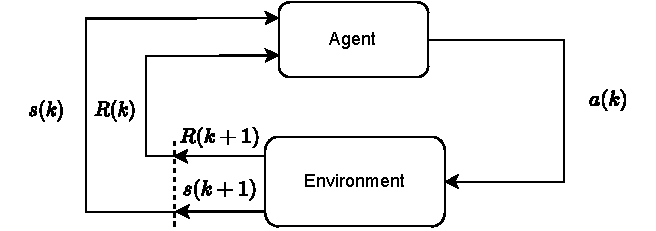
\includegraphics[width=1\linewidth]{Figures/AgentEnvironment.pdf}
	\caption{Interactions between agent and environment.}
	\label{fig:Agent-environment}
\end{figure}

The agent applies control action $ a(k) $ to the environment, based on the current state-combination $ s(k) $ and receives reward $ R(k+1) $, for bringing the environment to a new state $ s(k+1) $. The process is repeated until the state is terminal. The reinforcement learning sequence is: 

\begin{equation}
	s(0), a(0), R(1), s(1), a(1), R(2), s(2), a(2),\cdots	
\end{equation}

For discrete state and discrete action reinforcement learning: $ a(k)\in \mathcal{A} $, $s(k)\in \mathcal{S} $. That is, the available states and actions belongs to closed sets $\mathcal{S,A}$. And the reward $ R(k+1) \in \mathcal{R} \subset \mathbb{R} $. Notice that we take some notational freedom here, and exclude $s$ and $a$ from the $R$ notation, $R$ does inherently depend on state and action.

The agent seeks to maximise a series of rewards over time, called return $(G)$, through choices of actions \cite{Sutton2020}. Often a weighted sum of reward is used with $0 \leq \gamma \leq 1$:

\begin{equation}\label{eq:ExpectedReturn1}
	G(k)=R(k+1)
	+\gamma R(k+2)
%	+\gamma^{2}R(k+3)
	+\cdots
	+\gamma^{m}R(k+m+1)
	=\sum_{n=0}^{m}\gamma^{n}R(k+n+1)
\end{equation}

Where $ m $ is final time step of learning. In some problems learning is continuing and $m = \infty$. Learning problems with finite $m$ are called \textit{episodic}. This project deals with continuing learning, and we will use infinity throughout the report. 

By choosing $0 \leq \gamma < 1$ it ensures that higher importance is given to immediate reward rather than future rewards. Rewriting \cref{eq:ExpectedReturn1} to a recursive form yields:

\begin{equation}\label{eq:ExpectedReturn2}
	\begin{split}
			G(k)&=R(k+1)+\gamma R(k+2)+\gamma^2 R(k+3)+\cdots\\
			    &=R(k+1)+\gamma\big(R(k+2)+\gamma R(k+3)+\cdots\big)\\
			    &=R(k+1)+\gamma G(k+1)
	\end{split}
\end{equation}

The value function is defined as the expected return under a policy $ \mathbb{E}_{\pi} $, when starting in $a(k)$ state $ s(k) $ and afterwards following a policy $ \pi $ and is a measure of the \textit{value} of being in a state.   

%\begin{equation}\label{eq:IntroVfunc}
%		v_{\pi}(s)=\mathbb{E}_{\pi}\bigg[ %G(k) \big| s(k)=s\bigg]
%		%=\mathbb{E}_{\pi}\bigg[=R(k+1)+\gamma %G(k+1) \big| s(k)=s\bigg]
%\end{equation}

\begin{equation}\label{eq:IntroVfunc}
	v_{\pi}\bigg(s(k)\bigg)=\mathbb{E}_{\pi}\bigg[ G(k) \; \big|  \; s(k)\bigg]
	=\mathbb{E}_{\pi}\bigg[=R(k+1)+\gamma G(k+1) \; \big| \; s(k)\bigg]
\end{equation}

The policy $ \pi $ determines control actions, that is a mapping of the current state into an action - $ s(k) \mapsto a(k) $. $\pi$ is usually designed such that it selects actions resulting in highest expected return. Such a policy results in the optimal value-function:

%\begin{equation}
%	v_{\star}(s)=\underset{\pi}{\max} \; v_{\pi}(s)
%\end{equation}

\begin{equation}
	v_{\star}\bigg(s(k)\bigg)=\underset{\pi}{\max} \; v_{\pi}\bigg(s(k)\bigg)
\end{equation}

Since it is not realistic to maximise over all possible policies, we introduce the action value function in the pursuit of finding a different approach. The action value function is defined as the expected return when taking an action $ a(k) $ in a state $s(k)$ and afterwards following policy $\pi$:

%\begin{equation}\label{eq:IntroQfunc}
%	Q_{\pi}(s,a)=\mathbb{E}_{\pi}\bigg[ G(k) \big| s(k)=s,a(k)=a \bigg]
%	=\mathbb{E}_{\pi}\bigg[ R(k+1)+\gamma G(k+1) \big| s(k)=s,a(k)=a\bigg]
%\end{equation}

\begin{equation}\label{eq:IntroQfunc}
	Q_{\pi}\bigg(s(k),a(k)\bigg)=\mathbb{E}_{\pi}\bigg[ G(k) \; \big| \; s(k),a(k) \bigg]
	=\mathbb{E}_{\pi}\bigg[ R(k+1)+\gamma G(k+1) \; \big| \; s(k),a(k)\bigg]
\end{equation}

Optimal policies share same optimal action value functions which are defined as:

%\begin{equation}
%	Q_{\star}\bigg(s,a\bigg)=\underset{\pi}{\max} \; Q_{\pi}\bigg(s,a\bigg)
%\end{equation}

\begin{equation}
	Q_{\star}\bigg(s(k),a(k)\bigg)=\underset{\pi}{\max} \; Q_{\pi}\bigg(s(k),a(k)\bigg)
\end{equation}

$ Q_{\star} $ can be written in terms of $ v_{\star} $:

%\begin{equation}
%	Q_{\star}\bigg(s,a\bigg)=\mathbb{E}\bigg[R(k+1)+\gamma v_{\star}\bigg(s(k+1)\bigg) \big| s(k)=s,a(k)=a \bigg]
%\end{equation}

\begin{equation}
	Q_{\star}\bigg(s(k),a(k)\bigg)=\mathbb{E}\bigg[R(k+1)+\gamma v_{\star}\bigg(s(k+1)\bigg) \; \big| \; s(k),a(k) \bigg]
\end{equation}

This function computes the expected return for taking action $a(k)$ while being in state $s(k)$, and afterwards following an optimal policy. The entire value of following an optimal policy is contained in the optimal state value of the next state.

The optimal value of a state under an optimal policy must equal the expected return for the best action from that state. This action can be found by finding the action that yields the maximum value in the action value function.

%\begin{equation}
%	\begin{split}
%		v_{\star}\bigg(s\bigg)&=\underset{a'}{\max} \; Q_{\pi\star}\bigg(s,a'\bigg)\\
%					&=\underset{a'}{\max} \; \mathbb{E}_{\pi\star}\bigg[ R(k+1)+\gamma G(k+1) \big| s(k)=s,a(k)=a'\bigg]\\
%					&=\underset{a'}{\max} \; \mathbb{E}\bigg[ R(k+1)+\gamma v_{\star}\bigg(s(k+1)\bigg) \big| s(k)=s,a(k)=a'\bigg]\\
%					&=\underset{a'}{\max}\sum_{s'}p\bigg(s'|s(k),a'\bigg)\bigg[R(k+1)+\gamma v_{*}(s')\bigg]
%		\end{split}
%\end{equation}

\begin{equation}
	\begin{split}
		v_{\star}\bigg(s(k)\bigg)&=\underset{a'}{\max} \; Q_{\pi\star}\bigg(s(k),a'\bigg)\\
		&=\underset{a'}{\max} \; \mathbb{E}_{\pi\star}\bigg[ R(k+1)+\gamma G(k+1) \; \big| \; s(k),a'\bigg]\\
		&=\underset{a'}{\max} \; \mathbb{E}\bigg[ R(k+1)+\gamma v_{\star}\bigg(s(k+1)\bigg) \; \big| \; s(k),a'\bigg]\\
		&=\underset{a'}{\max}\sum_{s'}p\bigg(s' \; \big| \; s(k),a'\bigg)\bigg[R(k+1)+\gamma v_{*}(s')\bigg]
	\end{split}
\end{equation}

Where $ p(s'|s,a) $ is  probability of transition to state $ s' $, from state $ s(k) $ taking action $ a' $. The last equation is the Bellman optimality equation, see the next \cref{sec:Bellman}. Similarly the Bellman equation for the action value function can be written as:

%\begin{equation}
%	\begin{split}
%		Q_{\star}\bigg(s,a\bigg)&=\mathbb{E}\bigg[R(k+1) + \gamma \underset{a'}{\max} \; Q_{\star}\bigg(s(k+1),a'\bigg)\big|s(k)=s,a(k)=a\bigg]\\
%		&= \sum_{s'}p\bigg(s'|s(k),a(k)\bigg)\bigg[R(k+1)+\gamma \max_{a'}Q_{*}\bigg(s',a'\bigg)\bigg]
%	\end{split}
%\end{equation}

\begin{equation}
	\begin{split}
		Q_{\star}\bigg(s(k),a(k)\bigg)&=\mathbb{E}\bigg[R(k+1) + \gamma \underset{a'}{\max} \; Q_{\star}\big(s(k+1),a'\big) \; \big| \; s(k),a(k)\bigg]\\
		&= \sum_{s'}p\bigg(s'|s(k),a(k)\bigg)\bigg[R(k+1)+\gamma \max_{a'}Q_{*}\big(s',a'\big)\bigg]
	\end{split}
\end{equation}
 
\newpage

\section{The Bellman Equation} \label{sec:Bellman}
Here a more detailed look at the Bellman equation in its general from is presented. It lays the foundation for reinforcement learning solutions.  

\begin{equation}\label{eq:Bellman}
	v_{\pi}\bigg(s(k)\bigg)=\sum_{a'}\pi\bigg(a'|s(k)\bigg)\sum_{s'}p\bigg(s'|s(k),a'\bigg)\bigg[R(k+1)+\gamma v_{\pi}(s')\bigg]
\end{equation}

where,
\begin{center}
	\begin{tabular}{l p{12cm}}
		$v_{\pi}\bigg(s(k)\bigg) $ & is the  value of state $ s(k) $ under policy $ \pi $\\ 
		$ \pi\bigg(a'|s(k)\bigg) $ & is the conditional probability of taking action $ a' $ in state $ s(k) $ under stochastic policy $ \pi $\\
		$ p\bigg(s'|s(k),a'\bigg) $ & is the conditional probability of transitioning to state $ s' $ when taking action $ a' $ in state $ s(k) $ \\
%		$R(k+1)$ & is the reward for bringing the environment from $ s(k) \rightarrow s(k+1) $\\
	\end{tabular}
\end{center}

\hfill 

\cref{eq:Bellman} is the Bellman equation for the value function. The equation can be read as weighing the immediate reward and a discounted version of future state value by the probability of getting that reward and next state, when taking a specific action in a given state.  When summing over all possible actions and their possible next states an expression for the expected value of being in that state is obtained. In some versions of \cref{eq:Bellman} you also sum over all possible rewards, however, we assume it to be deterministic.

These optimality equations make systems of equations which can be solved, this is the Dynamic Programming approach. However, the set of equations are potentially unsolvable, and require a complete model of the system to know the transition probabilities. Therefore \cref{sec:TD-Methods} considers model-free estimation methods \textit{SARSA} and \textit{Q-learning}.

\section{Policies}

The simplest policy chooses actions based on the highest expected return achievable in a state $ s(k) $, that is, the highest action value:

\begin{equation}\label{eq:Greedy}
	a(k)=\underset{a'\in \mathcal{A}}{\arg\max} \; Q\bigg(s(k),a'\bigg)
\end{equation}

\cref{eq:Greedy} is called the \textit{greedy-policy}. The policy clearly takes advantage of already known information about the action values, this is known as \textit{exploitation}.

A greedy policy always chooses the action that it thinks is best at the current time, but this may result in convergence to a sub-optimal policy. The algorithm can get tunnel vision on a specific policy if it never checks other options, options which might yield better returns, especially in the long run. For example scenarios where multiple bad steps must be taken before a big reward is achieved. A greedy policy is also not able to detect changes in the environment. Allowing the agent to \textit{explore} new knowledge about the action value function can improve the agent's knowledge and lead to better decision making and performance. \cref{eq:EpsilonGreedy} presents the \textit{Epsilon-Greedy policy} which is a very simple method that balances exploration and exploitation by randomly choosing between the two options:

\begin{equation}\label{eq:EpsilonGreedy}
	a(k) = 
	\begin{cases} 
		\underset{a'\in \mathcal{A}}{\arg\max} \; Q\bigg(s(k),a'\bigg) & \text{exploitation with probability} \; 1-\epsilon  \\
		\text{Random action from $ \mathcal{A} $} & \text{exploration with probability} \; \epsilon 
	\end{cases},\quad \epsilon \in [0,1]
\end{equation}

If the $\epsilon$-value is chosen low \cref{eq:EpsilonGreedy} behaves greedy most of the time, but sometimes, instead of following the greedy-policy, it randomly chooses an action from the closed set of actions with equal probability independent of best action value. Doing this means the entire state-action space is explored as $ k \rightarrow \infty $. The downside is the immediate loss of reward from randomly choosing a worse action, this is especially noticeable as the algorithm gets closer to convergence, and shows the diminishing effectiveness of exploration.	

\section{Temporal Difference Methods}\label{sec:TD-Methods}
We choose to skip the topic of Monte Carlo simulation, as we wish to avoid its disadvantage of batch updating  - see e.g. \cite{Busoniu2010, Sutton2020} - and go directly to the topic of Temporal Difference learning. Temporal difference learning is a central idea of reinforcement learning. It makes it possible for the agent to learn while interacting with the environment for which no knowledge about the dynamics is known \cite{DaMottaSallesBarreto2008}, and in an iterative way finds the optimal action value function. It is also proven to converge to an optimal policy under the same conditions as other methods, and although temporal difference methods has not been proven to converge faster mathematically, empiric experiments show that temporal difference methods converge faster than Monte Carlo methods \cite{Sutton2020}.

SARSA is an abbreviation of State-Action-Reward-State-Action and forms the basis of TD(0) learning:

\begin{equation}\label{eq:sarsa}
	Q\bigg(s(k),a(k)\bigg)\leftarrow Q\bigg(
	s(k),a(k)\bigg)+\alpha	 
	\Bigg[
	\underbrace{R(k+1)+\gamma Q\bigg(s(k+1),a(k+1)\bigg)}_{\text{Temporal difference target/Sarsa target}}
	-Q\bigg(s(k),a(k)\bigg)
	\Bigg]
\end{equation}

Unlike Monte Carlo methods, Temporal Difference learning updates an action value after every iteration. This results in least amount of time spent on making sub-optimal actions. The method updates an estimate of the action value function based on the same estimate. This is called bootstrapping. 

Temporal Difference methods use \textit{sample updates} and therefore does not require a system model. This means looking ahead and combining the value at the next state-action pair and the reward obtained along the way, to compute a backed-up value for the current iteration (k), which is used to update the original state \cite{Sutton2020}.

One of the most used reinforcement learning method is called Q-learning, which like \cref{eq:sarsa} approximates the Bellman equation by updating the action value function iteratively  as seen in \cref{eq:Q-learning}.

\begin{equation}\label{eq:Q-learning}
	Q\bigg(s(k),a(k)\bigg)\leftarrow Q\bigg(s(k),a(k)\bigg)+\alpha \Bigg[
	\underbrace{R(k+1)+\gamma \max_{a'} 
		Q\bigg(s(k+1),a'\bigg)}_{\text{Q-Learning target}}
	-Q\bigg(s(k),a(k)\bigg)
	\Bigg]
\end{equation}

where,
\begin{center}
	\begin{tabular}{l p{12cm}}
		$ \alpha $ & is the \textit{Learning rate}. $0\leq \alpha \leq 1$. \\
	\end{tabular}
\end{center}

Note that the only difference in the two update methods lies in the target. This difference is called \textit{on-} and \textit{off-} policy, depending on whether the update is based on strictly staying on policy, meaning target action is selected according to policy (SARSA), or target action is chosen optimally, independent of policy (Q-learning). This essentially means that Q-learning converges to the optimal policy immediately, where SARSA converges to a less optimal policy which also consider the randomness of the $ \epsilon$-greedy policy, such that a \textit{safer} policy is obtained. Here safety means policies in which random actions can lead to large negative reward, achieve less value.

The learning rate $\alpha$ dictates the size of updates, but also affects if the algorithm can converge at all. The following properties on $ \alpha $ grantees convergence \cite{Busoniu2010}, such that if: 

\begin{equation}\label{eq:alphaAssumptions}
	\sum_{k=1}^{\infty}\alpha(k)=\infty \quad \wedge \quad \sum_{k=1}^{\infty}\alpha(k)^{2}<\infty
\end{equation} 

Then: 

\begin{equation}
	Q(s,a) \rightarrow Q_\star(s,a)\hspace{0.108cm} \text{as}\hspace{0.108cm}k \rightarrow\infty,\hspace{0.108cm} \forall s,a \in \mathcal{S,A}
\end{equation}

Where $ Q_{\star} $ denotes the optimal action value function. The first condition in \cref{eq:alphaAssumptions} is required to guarantee that the steps are large enough to eventually
overcome any initial conditions or random fluctuations. The second condition guarantees
that eventually the steps become small enough to assure convergence \cite{Sutton2020}.

\section{Function Approximation}\label{sec:FuncApprox}
One way of keeping track of the action values is to use a table. For large systems with high state-action dimensionality this is not desirable. The agent is required to visit all state-action combinations at least once to get an idea of optimal decision making. Visiting the whole state-action space could take an enormous amount of time resulting in long learning periods and convergence times.

Instead the action value function can be approximated \cite{Sutton2020}. This allows us to generalise information about visited state-actions pairs to not yet visited pairs:

\begin{equation}\label{eq:QApprox1}
	\hat{Q}\bigg(s(k),a(k),\textbf{w}\bigg) \approx Q_{\pi}\bigg(s(k),a(k)\bigg)
\end{equation}

The state-action function estimate is now represented as a parametrised function form with a weight vector $ \textbf{w} \in \mathbb{R}^{d}$. The linear\footnote{Linear with respect to weights} approximation of the action-value function is given by:

\begin{equation}\label{eq:QApprox2}
	\hat{Q}\bigg(s(k),a(k),\textbf{w}\bigg)=\textbf{w}^{\intercal}\textbf{x}\bigg(s(k),a(k)\bigg)=\sum_{i=1}^{d}w_{i}x_{i}\bigg(s(k),a(k)\bigg)
\end{equation}

Where 

\begin{equation}
	\textbf{x}\bigg(s(k),a(k)\bigg) = \bigg[x_{1}\bigg(s(k),a(k)\bigg), x_{2}\bigg(s(k),a(k)\bigg) \cdots x_{d}\bigg(s(k),a(k)\bigg)\bigg]^\intercal
\end{equation}
 
is the feature vector and each element $ x_{i} $ is called a feature of the states.

The weight vector is updated using stochastic gradient descent, which minimises the squared error between the true state-action function and the estimated function \cite{Overgaard2019}:

\begin{equation}\label{eq:QApprox3}
	\begin{split}
		\textbf{w} 
		& \leftarrow\textbf{w}-\frac{1}{2}\alpha\nabla_{\textbf{w}}\big[Q_{\pi}\bigg(s(k),a(k)\bigg)-\hat{Q}\bigg(s(k),a(k),\textbf{w}\bigg)\bigg]^{2}\\
		&=\textbf{w}+\alpha\bigg[Q_{\pi}\bigg(s(k),a(k)\bigg)-\hat{Q}\bigg(s(k),a(k),\textbf{w}\bigg)\bigg]\nabla_{\textbf{w}}\hat{Q}\bigg(s(k),a(k),\textbf{w}\bigg)
	\end{split}
\end{equation}


$\alpha$ is a positive step size, and $\nabla_{\textbf{w}} \hat{Q}\bigg(s(k),a(k),\textbf{w}\bigg)$ is the gradient of the function $ \hat{Q} $ with respect to the weight vector $ \textbf{w} $. \cref{eq:QApprox3} requires that the actual action value function $ Q_{\pi} $ is known which is typically not the case. An estimate, $ U $, of $ Q_{\pi}\bigg(s(k),a(k)\bigg) $ is used:

\begin{equation}\label{eq:QApprox5}
	\textbf{w}_{} \leftarrow \textbf{w}_{}+\alpha\bigg[U-\hat{Q}\bigg(s(k),a(k),\textbf{w}\bigg)\bigg]\nabla\hat{Q}\bigg(s(k),a(k),\textbf{w}\bigg)
\end{equation}

Choosing the estimate as in \cite{Overgaard2019,Sutton2020}: 

\begin{equation}\label{eq:SSGDtarget}
	U = R(k+1)+\gamma \max_{a'}\hat{Q}\bigg(s(k+1),a',\textbf{w}\bigg)
\end{equation}

Combining \cref{eq:QApprox5} and \cref{eq:SSGDtarget} yields the update law for the weight vector:

\begin{equation}\label{eq:QApprox6}
	\textbf{w} \leftarrow \textbf{w}
	+\alpha\bigg[R(k+1)+\gamma\max_{a'}\hat{Q}\bigg(s(k+1),a',\textbf{w}\bigg)
	-\hat{Q}\bigg(s(k),a(k),\textbf{w}\bigg)\bigg]\nabla_{\textbf{w}}\hat{Q}\bigg(s(k),a(k),\textbf{w}\bigg)
\end{equation}

Evaluating $ \nabla_{\textbf{w}}\hat{Q}\bigg(s(k),a(k),\textbf{w}\bigg) $ in \cref{eq:QApprox2} yields:

\begin{equation}\label{eq:NablaQApprox}
\begin{split}
		\nabla_{\textbf{w}}\hat{Q}\bigg(s(k),a(k),\textbf{w}\bigg) 
		&=\nabla_{\textbf{w}}\bigg(\textbf{w}^{\intercal}\textbf{x}\bigg(s(k),a(k)\bigg)\bigg)\\
	&=\textbf{x}\bigg(s(k),a(k)\bigg)
\end{split}
\end{equation}

\cref{eq:QApproxFinal} presents the semi-gradient descent update rule for function approximation: 

\begin{equation}\label{eq:QApproxFinal}
	\textbf{w} \leftarrow \textbf{w}
	+\alpha\bigg[R(k+1)+\gamma\max_{a'}\hat{Q}\bigg(s(k+1),a',\textbf{w}\bigg)
	-\hat{Q}\bigg(s(k),a(k),\textbf{w}\bigg)\bigg]\textbf{x}\bigg(s(k),a(k)\bigg)
\end{equation}

\newpage

\chapter{Water Distribution Networks}\label{chap:WDN}
A water distribution network is a hydraulic network which consists of different components; pipes, pumps, valves and elevated water reservoirs. The network is usually divided into several consumer zones. A ring-type water distribution network can be seen in \cref{fig:WDNintro} with two consumer zones, two pumping stations, and an elevated water reservoir. As mentioned in \cref{sec:introMotivation} the purpose of an elevated water reservoir is to maintain pressure, but also to store water in case of an emergency. When the pressure is high in the network but the demand is low, water will flow into the reservoir and vice-versa. But from an economic viewpoint it is desired to keep the pumps running as little as possible resulting in lower water levels in the reservoir. Efficient operation of the water distribution network inherently means minimising energy usage, which extends efficient operation to also impact the green transition \cite{Val2021a}.
 
 \begin{figure}[h!]
	\centering
	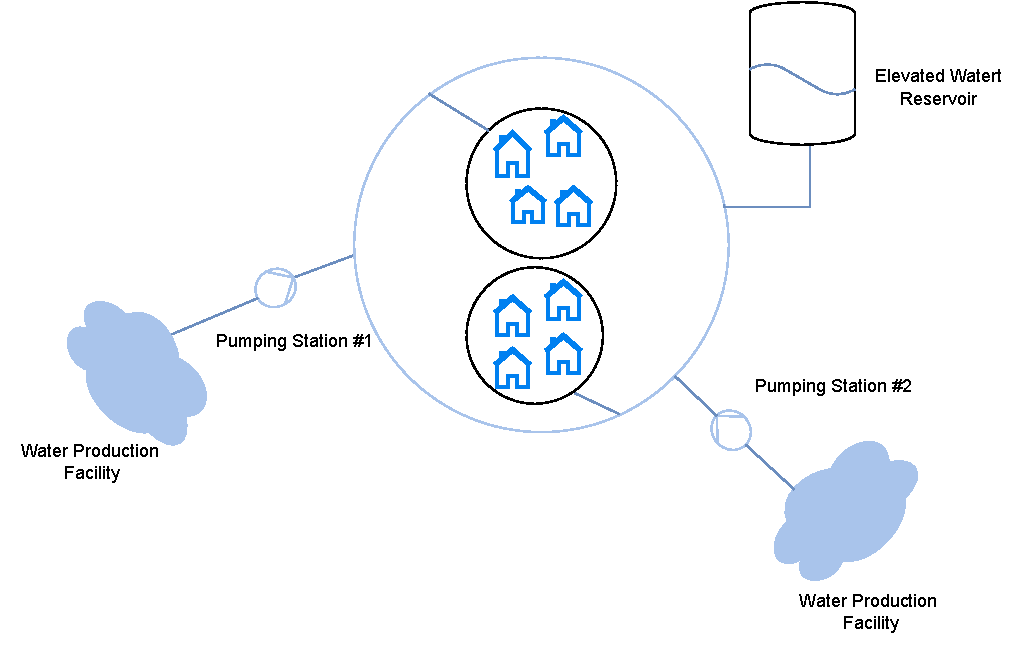
\includegraphics[width=0.6\linewidth]{Figures/WDNintro.pdf}
	\caption{A typical ring-type water distribution network with two pumping stations, multiple consumers and an elevated reservoir.}
	\label{fig:WDNintro}
\end{figure}

In order to verify the methods of this project are applicable in the real world, they are implemented on a water distribution network test setup.
  
\section{Test Setup}\label{sec:WDNsetup}
\cref{fig:WDN} presents the water distribution network test setup used in the project. The system consists of three parallel coupled pumps, acting as a pumping station which supplies water to a variable valve acting as a consumer zone, and an elevated water reservoir. For a comprehensive overview of component models in water distribution see \cite{Jensen}.

 \begin{figure}[h!]
	\centering
	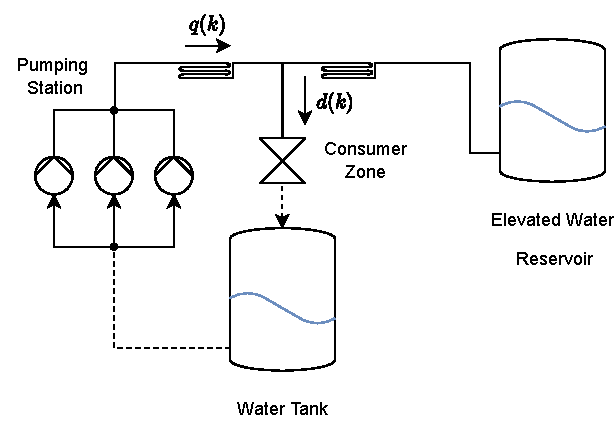
\includegraphics[width=0.81\linewidth]{Figures/WDN}
	\caption{Water distribution network with pumping station, consumer zone and elevated water reservoir.}
	\label{fig:WDN}
\end{figure}

The water tank is used to store water for the pumping station and is kept at a constant level with the help of a PI-controller that controls a set of auxiliary pumps.

The only dynamic component of the network seen in \cref{fig:WDN} is the elevated water reservoir, and can be described by the following differential equation:

\begin{equation}\label{eq:hDynamic}
	A\dot{h} = q + d \Leftrightarrow \dot{h} = \frac{q+d}{A}
\end{equation}  

\cref{eq:hDynamic} can be discretized by Euler's method:

\begin{equation}
	h(k+1) = h(k) + \frac{q(k)+d(k)}{A} 
\end{equation}

where,
\begin{center}
	\begin{tabular}{l p{10cm} l}
		$ h(k) $ & is the water level in the elevated water reservoir & [\si{m}]\\
		$ q(k) $ & is the flow of water through the pumps & [\si{m\cubed}/\si{s}]\\
		$ d(k) $ & is the water demand & [\si{m\cubed}/\si{s}]\\
		$ A $ & is the cross-sectional area of the elevated water reservoir & [\si{m\squared}]
	\end{tabular}
\end{center}

Note that the cross-sectional area of the elevated water reservoir is assumed constant along its vertical axis. \cite{Rathore930,MathiasJeppe730} uses the same elevated water reservoir as this project and states the following parameters:

\begin{table}[h!]
	\centering
	\begin{tabular}{|c|c|c|c|}
		\hline
		Diameter [\si{m}] & Height [\si{m}] & Cross sectional area [\si{m\squared}] & Capacity [\si{m\cubed}] \\ \hline
		0.6      & 0.706  & 0.283                & 0.2      \\ \hline
	\end{tabular}
	\caption{Elevated water reservoir parameters. Cross sectional is used in simulation.}
	\label{tab:Tank Parameters}
\end{table}

The power delivered to the water from the pumping station in \cref{fig:WDN} is:

\begin{equation}
			P(k) = q(k)\Delta{p}= q(k)(p_{out}(k)-p_{in}(k))
\end{equation}

Where the system pressure $ p_{out} $ is:

\begin{equation}
	p_{out}(k)=\rho g h_{ewr}(k)+\Delta{z}+\lambda_{1}\bigg(q(k)\bigg)+\lambda_{2}\bigg(q(k),d(k)\bigg)
\end{equation}

where,
\begin{center}
	\begin{tabular}{l p{10cm} l}
		$ \rho $ & is the density of water & [\si{l/m^{3}}]\\
		$ g $ & is the gravitational acceleration & [\si{m/s^{2}}]\\
		$\Delta{z}$ & is the drop in pressure due to geodesic level of tank & [\si{Pa}]\\
		$\lambda(\mathord{\cdot})$ & is the drop in pressure due to friction in a pipe-segment & [\si{Pa}] \\
		$p_{out},p_{in}$ & are the absolute pressure at outlet and inlet side of pumping station & [\si{Pa}]\\
	\end{tabular}
\end{center}

It is assumed that the pressure drop in the pipe connected to the pumping station, due to friction, takes the form: 

\begin{equation}
	\lambda_{1}\bigg(q(k)\bigg) = r_{1}\big|q(k)\big|q(k)
\end{equation}

and for a pipe connected to an elevated water reservoir the pressure drop takes the form: 

\begin{equation}
	\lambda_{2}\bigg(q(k),d(k)\bigg) = r_{2}\big|q(k)-d(k)\big|\bigg(q(k)-d(k)\bigg) 
\end{equation}

with friction constants $ r_{i} $.

The pump inlet is assumed open to atmosphere and the inlet pressure becomes $p_{in} = 0$. The power delivered from the pumping station is:

\begin{equation}\label{eq:WDN_Power}
P(k)= q(k)\bigg(\rho g h_{ewr}(k)+\Delta{z}+\lambda_{1}\bigg(q(k)\bigg)+\lambda_{2}\bigg(q(k),d(k)\bigg) \bigg) 
\end{equation}
 
\section{Consumption Model}\label{sec:Consumption}
Real water consumption data is analysed. A historical dataset of daily water consumption over a three months period has been provided by Grundfos, which contains data sampled four times per hour. \cref{fig:Consumption} depicts consumption of a 24 hour period. Note that the unit of the consumption data is unknown and that \cref{fig:Consumption} is normalised. 

\begin{figure}[h!]
	\centering
	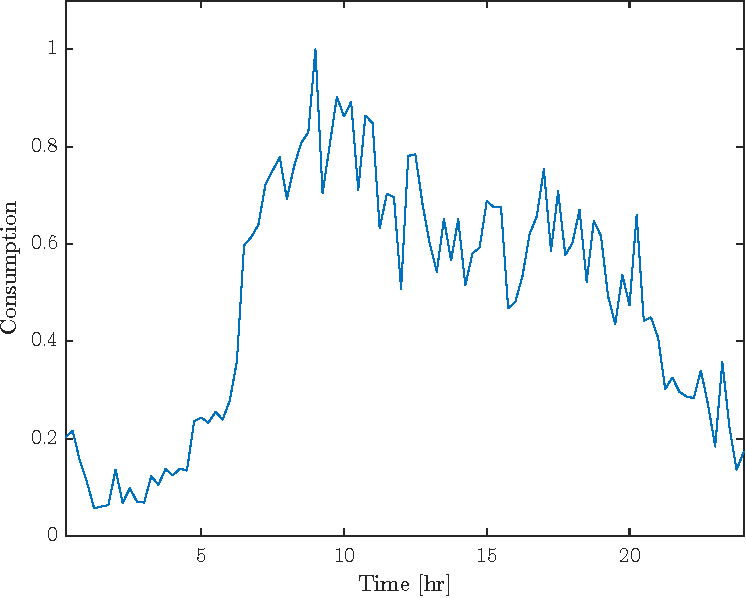
\includegraphics[width=0.7\linewidth]{Figures/Consumption.pdf}
	\caption{Consumption profile in a day.}
	\label{fig:Consumption}
\end{figure}

The power equation presented in \cref{eq:WDN_Power} will in the following section be used to select states and action of the system, such that reinforcement learning can be used as a control method. The consumer data will be used to emulate the consumption of a consumer zone, and will play a role when doing full state function approximation Q-learning.

\newpage

\chapter{Water Distribution Networks and Reinforcement Learning}\label{chap:RLOnWDN}

In this chapter it is shown how reinforcement learning methods from \cref{chap:RL} are used as control methods on the water distribution network presented in \cref{chap:WDN}. A cost function is formulated based on minimisation of energy consumption of pumps, combined with a barrier function. System states and action is selected based on the cost function.

\cref{chap:RL} describes two learning algorithms; the on-policy learning method Sarsa and the off-policy learning method Q-learning. The Sarsa algorithm \cref{eq:sarsa} will in time learn the optimal $ \epsilon $-greedy policy, that is the Q-values will converge to some sub-optimal Q-value function. Using Q-learning will result in the convergence to an optimal policy \cite{Sutton2020}, therefore the Q-learning algorithm will be used for the remainder of the project.  

Notice from here onward, we distinguish between the height state and actual water level height, by denoting them $h(k)$ and $h_{ewh}(k)$ respectively.

\newpage \clearpage

\section{Cost Function and State-Action Selection}\label{sec:CostFuncAndState-ActionSelection}
\cref{chap:RL} presented Reinforcement Learning and the idea of maximisation a reward function to get the greatest return. The remainder of this project will discuss minimization of a cost functions rather than maximisation of a reward functions. This means that the action value becomes related to an expected cost for which lower values are better. The $\epsilon$-greedy policy should then be altered such that the next action is found based on lowest action value rather than the biggest action value:

\begin{equation}\label{eq:EpsilonGreedyMin}
	a(k) = 
	\begin{cases} 
		\underset{a'\in A}{\arg\min} \; Q\bigg(s(k),a'\bigg) & \text{exploitation with probability} \; 1-\epsilon  \\
		\text{Random action from $ \mathcal{A} $} & \text{exploration with probability} \; \epsilon 
	\end{cases},\quad \epsilon \in [0,1]
\end{equation}

The cost function $ J $ forms the basis of the optimality problem. We formulate the cost function such that the power consumed by the pumping station is minimised and on the fact that we wish to stay within some water level limits in the elevated water reservoir:

\begin{equation}\label{eq:WDN_Cost1}
	J(k+1) = P(k) + B\bigg(h_{ewr}(k+1)\bigg)  
\end{equation}  

where,
\begin{center}
	\begin{tabular}{l p{10cm} l}
		$ P(k) $ & is the power consumed by the pumping station & [\si{W}]\\
		$ B\bigg(h_{ewr}(k+1)\bigg) $ & is a barrier function & ($\cdot$)
	\end{tabular}
\end{center}

Note that the cost is based on pump power at time $ k $ and the barrier cost is evaluated at time $ k+1 $ resulting in high cost given to actions that takes the water level into the barrier. Combining \cref{eq:WDN_Cost1} and \cref{eq:WDN_Power} yields:

\begin{equation}\label{eq:CostFunctionFinal}
	J(k+1)= q(k)\bigg(\rho g h_{ewr}(k+1)+\Delta z+\lambda\bigg(q(k)\bigg)+\lambda \bigg(q(k),d(k) \bigg)\bigg) + B\bigg(h_{ewr}(k+1)\bigg) 
\end{equation}

The barrier function is  designed such that high costs is given to water levels that are outside certain heights bounds. The barrier helps in avoiding dry-out, this is important since it counteracts the minimisation of energy inclination to empty the reservoir. Avoiding dry-out also guarantees that demand will be satisfied, because demand will drain the reservoir if pumps supply insufficient water. 

%As such the barrier function counteracts the cost of using pump power, this cost-balance determined by how the barrier is designed is one of the primary tools to shape the stationary behaviour of the system.

\cref{eq:QuadBarrier} presents the quadratic polynomial barrier function used: 

%A barrier function is included in the cost function adding a high cost to the extreme upper and lower areas of the operating range of the reservoirs water level. This is a first step toward safe learning, partly safeguarding against overflow and dryout, 

\begin{equation}\label{eq:QuadBarrier}
	B\bigg(h_{ewr}(k),a,b\bigg)=\begin{cases}
		(h_{ewr}(k)-a)^{2} & \text{if} \; h_{ewr}(k) < a \\
		0 & \text{if} \; h_{ewr}(k)\in\big[a,b\big] \\
		(h_{ewr}(k)-b)^2 & \text{if} \; h_{ewr}(k) > b 
	\end{cases}
\end{equation}

With $ a $ and $ b $ being the zeros of the left and right side polynomial respectively. A example of a barrier function of this form is shown in  \cref{fig:QuadBarrierFunc1}:

\begin{figure}[h!]
	\centering
	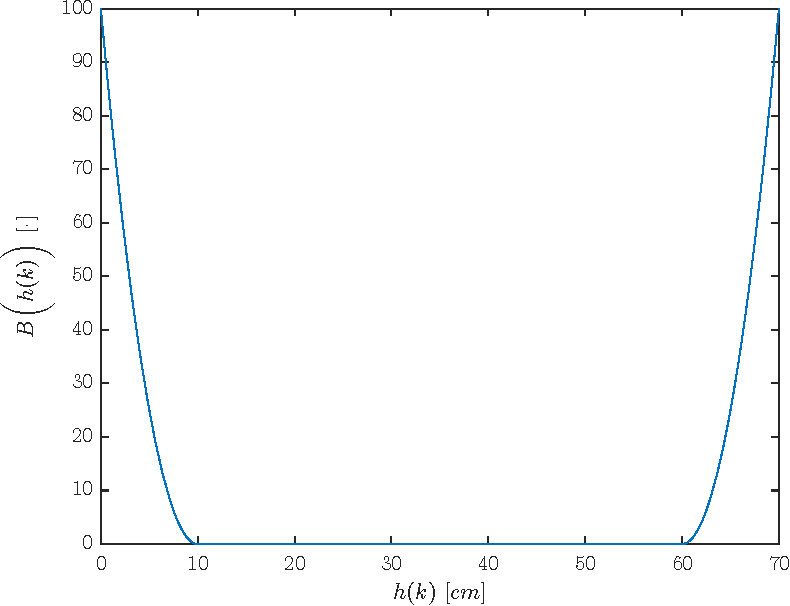
\includegraphics[width=0.7\linewidth]{Figures/QuadBarrierFuncA10B60}
	\caption{Piecewise defined quadratic barrier function from \cref{eq:QuadBarrier} with zeros in 10 and 60.}
	\label{fig:QuadBarrierFunc1}
\end{figure} 

States and action for the water distribution network reinforcement learning problem is chosen based on the cost function in \cref{eq:CostFunctionFinal}. We choose:

\begin{itemize}
	\item $ s_{1}  = h_{ewr}$: Water level of tank scales linearly to the pressure in the tank, and determines barrier cost.
	
	\item $ s_{2} = t $: Time of day. It is assumed that the consumer demand $d(k)$ behaves periodically from day to day.
	
	\item $ a = q(k) $: actions are three unique pumping-station presets, each with a different resulting flow. 
\end{itemize}


\newpage \clearpage

\section{Tabular Q-learning}\label{sec:WDNTabularQ-Learning}

For tabular Q-Learning the action values are stored in a table format: $ Q\bigg(h(k),t(k),a(k)\bigg) $. One table dimension holds discrete height states, one discrete time states and one discrete actions. 

\begin{wrapfigure}{r}{7.5cm}
	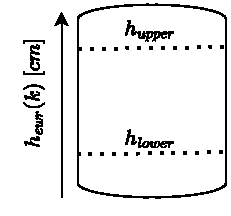
\includegraphics[width=7.5cm]{figures/HeightStates - Copy.drawio.pdf}
	\caption{Height state in elevated water reservoir.}
	\label{fig:hState}
\end{wrapfigure} 

This section explains how the states are discritised in order to fit the water distribution network described in \cref{chap:WDN}. 

Time is discretised to 24 states, matching hours of the day. A finer discretisation is not used for dimensionality issues, and it is assumed dynamics are slow enough to be captured on a hourly basis.

Discretisation of water levels in the elevated water reservoir is visualised in \cref{fig:hState}. The first and last height states consists of wider height segments than the middle states. This minimises the chance of dry-out and overflow. The water level is measured in centimetres and the height state $ h(k) $ will be chosen based on the actual water level: 

%\begin{equation} \label{eq:HeightStates}
%	h(k)=\begin{cases}
%		h_{1} & if \; h_{ewr}(k) \leq h_{Lower} \\
%		ceil\bigg(h_{ewr}(k)\bigg) & if \; h_{lower} < h_{ewr}(k) <h_{upper} \\
%		h_{n} & if \; h_{ewr}(k) \geq h_{upper} 
%	\end{cases}
%\end{equation}

\begin{equation} \label{eq:HeightStates}
	h(k)=\begin{cases}
		1 & if \; h_{ewr}(k) \leq h_{Lower} \\
		ceil\bigg(h_{ewr}(k)\bigg) & if \; h_{lower} < h_{ewr}(k) <h_{upper} \\
		h_{max} & if \; h_{ewr}(k) \geq h_{upper} 
	\end{cases}
\end{equation}

%Where $ h_{lower} $ and $ h_{upper} $ decide the region size of $ h_1 $ and $ h_n $ relative to the tank size and thereby the number of height states. $ ceil $ denotes the \textit{ceiling} function. 

Where the placements of $ h_{lower} $ and $ h_{upper} $ decide the number of height states, and the resulting upper limit of height states is denoted $ h_{max} $. $ ceil $ denotes the \textit{ceiling} function, which rounds any number to the nearest larger integer. Our use of the ceil function requires the argument to be measured in centimetres for proper height state assignment, therefore any measurement not in centimetres must first be scaled.

The number of actions is dictated by the number of pumps in the pumping station, and is by nature already discrete.

The Q-learning update law for the action value function described in \cref{eq:Q-learning} will in the case of minimising the cost function in \cref{eq:WDN_Cost1} be:

\begin{equation}\label{eq:Q-learningMin}
	\begin{split}
		Q\bigg(h(k),t(k),a(k)\bigg)\leftarrow Q\bigg(h(k),t(k),a(k)\bigg)&+\alpha \bigg[J(k+1)	+\gamma \min_{a'} Q\bigg(h(k+1),t(k+1),a'\bigg)\\
		&-Q\bigg(h(k),t(k),a(k)\bigg)\bigg]
	\end{split}
\end{equation}

with $ h(k) \in \mathcal{H} $, $ t(k) \in \mathcal{T}$ and $ a(k) \in \mathcal{A} $. That is the available states and actions belongs to closed sets. 

\cref{alg:Q-learning} presents the tabular Q-learning algorithm applied to the water distribution network presented in \cref{sec:WDNsetup}.

\begin{algorithm}
	\caption{Tabular Q-Learning algorithm}
	\label{alg:Q-learning}
	\begin{algorithmic}[1]
		\State \textbf{Input:} $\alpha\in[0,\;1]$, small $\epsilon>0$, and $0\leq\gamma < 1$ 
		\State \textbf{Initialise:} $ Q(h,t,a) $ for all $ h(k) \in \mathcal{H} $, $ t(k) \in \mathcal{T}$ and $ a(k) \in \mathcal{A} $, and states $ t(1) $ and $ h(1) $ 
		\For{k=1,2,...}
		\State Take action according to $\epsilon$-greedy policy:
		\begin{equation*}
			a(k) = \begin{cases} 
				\underset{a'\in \mathcal{A}}{\arg\min} \; Q\bigg(h(k),t(k),a'\bigg) & \text{exploitation with probability} \; 1-\epsilon  \\
				\text{Random action from $ \mathcal{A} $} & \text{exploration with probability} \; \epsilon 
			\end{cases}
		\end{equation*}
	\State Observe next states $ h(k+1) $, $ t(k+1) $ and cost $ J(k+1)$ 
	\State Update $ Q $ according to:
		\begin{equation*}
		\begin{split}
			Q\bigg(h(k),t(k),a(k)\bigg)\leftarrow &Q\bigg(h(k),t(k),a(k)\bigg)+\alpha \bigg[J(k+1)+\gamma \min_{a'} Q\bigg(h(k+1),t(k+1),a'\bigg)\\
			&-Q\bigg(h(k),t(k),a(k)\bigg)\bigg]
		\end{split}
	\end{equation*}
		\EndFor
	\end{algorithmic}
\end{algorithm}



\section{Function Approximation Q-learning}\label{sec:WDNFunctionApproximationQ-Learning}

To ease notation, and since the following sections does not require discretised height state, we will once again denote the actual water level as $h(k)$.

\cref{sec:FuncApprox} established that the action value function could be approximated as a linear combination of a weights vector and a set of basis functions:

\begin{equation}
	\hat{Q}\bigg(s(k),a(k),\textbf{w}\bigg)=\textbf{w}^{\intercal}\textbf{x}\bigg(s(k),a(k)\bigg)
\end{equation}

Applying function approximation to the water distribution network described in \cref{chap:WDN} with states and actions chosen as in \cref{sec:CostFuncAndState-ActionSelection} yields: 

\begin{equation}
	\hat{Q}\bigg(h(k),t(k),a(k),\textbf{w}\bigg)=\textbf{w}^{\intercal}\textbf{x}\bigg(h(k),t(k),a(k)\bigg)
\end{equation}

The approximation shown above is true for the case where all states and actions are continuous which is not the case for this project. This section shows how to deal with the following cases of continuous/discrete states and action combinations:

\begin{itemize}
	\item Continuous water level, and discrete time and action.
	\item Continuous water level and time, and discrete action.
\end{itemize} 

\subsection{Continuous Height, and Discrete Time and Action}\label{sec:WDN1D}

In the continuous height, and discrete time and action case we have $ s = (t,h) $ where $ t $ is in a finite set and $ h $ is continuous. It is necessary to create a weight-vector for every time-action combination. The action-value function will be approximated as:

\begin{equation}\label{eq:Qhat2Discrete}
	\hat{Q}\bigg(h(k),\textbf{w}_{t(k),a(k)}\bigg)=\textbf{w}_{t(k),a(k)}^{\intercal}\textbf{x}\bigg(h(k)\bigg)
\end{equation} 

The subscripts of $ \textbf{w} $ refer to one specific weight vector. There exists one weight vector for each discrete time, discrete action combination: For the case of $ 24 $ discrete times and $ 3 $ discrete actions there exist $ 96 $ weight vectors.

Radial basis functions are used for the height feature vector. They are easy to design and provide good generalisation due to their Gaussian bell shapes:

\begin{equation}\label{eq:RBF}
	x_{i}\bigg(h(k)\bigg) = \exp\bigg(\frac{-||h(k)-c_{i}||^2}{2\sigma_{i}^2}\bigg)
\end{equation}

The radial basis function is shaped by the feature's width $ \sigma_{i} $, and the feature response depends only on the distance to the state center $ c_{i} $ \cite{Sutton2020}. \cref{fig:RBF1D} shows radial basis functions in one dimension:

\begin{figure}[h!]
	\centering
	\includegraphics[width=0.8\linewidth]{Figures/RBF.pdf}
	\caption{Radial basis functions in one dimension \cite{Sutton2020}.}
	\label{fig:RBF1D}
\end{figure}

10 centers are placed uniformly in the range of $ 0 $ to $ 70\si{cm} $ according the the elevated water reservoir height presented in \cref{tab:Tank Parameters}:

\begin{equation*}
	c = \begin{bmatrix}
		0 & 7.78  & 15.56 &  23.33 &  31.11 &  38.89 &  46.67 &  54.44  & 62.22  & 70\\
	\end{bmatrix}
\end{equation*}

An even radial basis function generalisation is achieved by choosing $\sigma = 4$ such that the sum of radial basis functions equals one over the entire range of elevated water reservoir heights. The individual radial basis function is plotted in \cref{fig:RadialSum} along with the sum of all radial basis functions. 

\begin{figure}[h!]
	\centering
	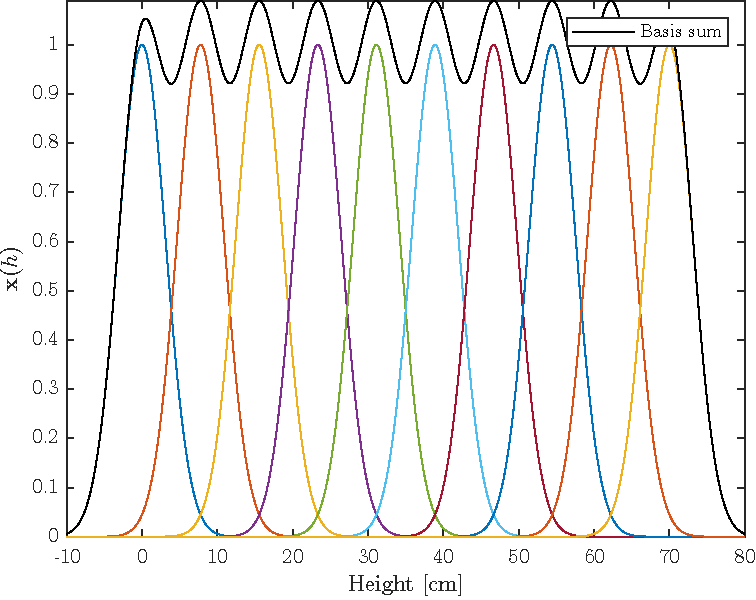
\includegraphics[width=0.7\linewidth]{Figures/RadialSum.pdf}
	\caption{Radial basis functions and their sum.}
	\label{fig:RadialSum}
\end{figure}

The weight vectors update rule will in the continuous height, discrete time and action case be: 

\begin{equation}
	\begin{split}
			\textbf{w}_{t(k),a(k)} \leftarrow \textbf{w}_{t(k),a(k)}
		&+\alpha\bigg[J(k+1)+\gamma\min_{a'}\bigg(\textbf{w}_{t(k+1),a'}^{\intercal}\textbf{x}\bigg(h(k+1)\bigg)\bigg)\\
		&-\textbf{w}_{t(k),a(k)}^{\intercal}\textbf{x}(h\bigg(k)\bigg)
		\bigg]\textbf{x}\bigg(h(k)\bigg)
	\end{split}
\end{equation}

Where $ t(k) $ and $ a(k) $ is taken from finite sets. \cref{alg:FuncApproxQ-learning} presents the function approximation Q-Learning algorithm applied to the water distribution network shown in \cref{sec:WDNsetup}. with continuous height state and discrete time state and discrete actions.

\begin{algorithm}
	\caption{Continuous height discrete time and action Function approximation Q-Learning algorithm}
	\label{alg:FuncApproxQ-learning}
	\begin{algorithmic}[1]
		\State \textbf{Input:} $\alpha\in[0,\;1]$, small $\epsilon>0$, and $0\leq\gamma < 1$, number of Radial basis functions, center placements and width
		
		\State \textbf{Initialise:} weight vectors $ \textbf{w}_{t,a} $ for all discrete times and actions (e.g. $ \textbf{w}_{t,a}=0 $), and states $ t(1) $ and $ h(1) $ 
		
		\For{k=1,2,...}

	\State Take action according to a $\epsilon$-greedy policy:
	\begin{equation*}
		a(k) = \begin{cases} 
			\underset{a'\in \mathcal{A}}{\arg\min} \; \hat{Q}\bigg(h(k),\textbf{w}_{t(k),a'}\bigg) & \text{exploitation with probability} \; 1-\epsilon  \\
			\text{Random action from $ \mathcal{A} $} & \text{exploration with probability} \; \epsilon 
		\end{cases}
	\end{equation*}

\State Observe next states $ h(k+1) $, $ t(k+1) $ and cost $ J(k+1) $

\State Update $ \textbf{w}_{t(k),a(k)} $ according to:
	\begin{equation*}
	\begin{split}
		\textbf{w}_{t(k),a(k)} \leftarrow \textbf{w}_{t(k),a(k)}
		&+\alpha\bigg[J(k+1)+\gamma\min_{a'}\bigg(\textbf{w}_{t(k+1),a'}^{\intercal}\textbf{x}\bigg(h(k+1)\bigg)\bigg)\\
		&-\textbf{w}_{t(k),a(k)}^{\intercal}\textbf{x}\bigg(h(k)\bigg)
		\bigg]\textbf{x}\bigg(h(k)\bigg)
	\end{split}
\end{equation*}
		\EndFor
	\end{algorithmic}
\end{algorithm}

\clearpage \newpage

\subsection{Continuous Height and Time, and Discrete Action}\label{sec:WDN2D}

In the continuous water level and time, and discrete action case, it is necessary to create a weight-vector for every discrete action. 

\begin{equation}\label{eq:Qhat1Discrete}
	\hat{Q}\bigg(h(k),t(k),\textbf{w}_{a}\bigg)=\textbf{w}_{a(k)}^{\intercal}\textbf{x}\bigg(h(k),t(k)\bigg)
\end{equation}

This reduces the number of weight vectors from 96 as in \cref{sec:WDN1D} to only 3. As in \cref{sec:WDN1D} radial basis functions are used as basis function for the height part of the feature vector. Another linear function approximation method is based on Fourier series, which are useful for approximating periodic functions such as water consumption:

\begin{equation}\label{eq:FSApproxDef}
	f(t)=a_{0}+\sum_{n=1}^{n=N}(a_{n}\cos(2\pi n f_{0} t)+b_{n}\sin(2\pi n f_{0}t))
\end{equation}

Where $ a_0, a_{n} $ and $ b_{n} \in \mathbb{R}$ are the Fourier coefficients and $ f_0 $ is the first harmonic of the signal. \cref{eq:FSApproxDef} can be rewritten as a linear combination of weights $ \textbf{w} $ and a feature vector $ \textbf{x} $ containing $\sin$ and $\cos$ basis functions.

\begin{equation}
	f(t)=\textbf{w}^\intercal\textbf{x}(t)
\end{equation}

With weight vector and basis functions defined as:

\begin{equation}\label{eq:wxFS}
	\textbf{w} = 
	\begin{bmatrix}
		a_{0}\\
		a_{1}\\
		b_{1}\\
		a_{2}\\
		\vdots
	\end{bmatrix}
\quad \wedge \quad
	\textbf{x}(t) = 
	\begin{bmatrix}
		1\\
		\sin(2\pi f_0 t)\\
		\cos(2\pi f_0 t)\\
		\sin(4\pi f_0 t)\\
		\vdots \\
	\end{bmatrix} 
\end{equation}

The harmonic frequencies found is based on a fast Fourier transformation of the consumer data described in \cref{sec:Consumption}. From the fast Fourier transform, shown in \cref{fig:FFT}, the demand profile is found to have a major dc-component and frequency-components corresponding to periods of 24 hours, 12 hours, 8 hours, 6 hours, and 4 hours corresponding to the first, second, third, fourth and sixth harmonic. 
 
\clearpage
\begin{figure}[h!]
	\centering
	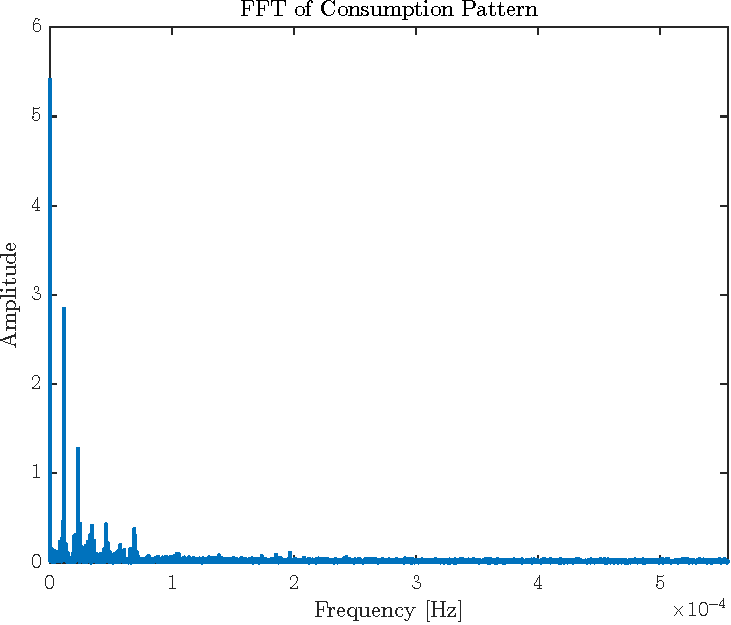
\includegraphics[width=0.7\linewidth]{Figures/FFT.pdf}
	\caption{Fast fourier transformation for consumer data.}
	\label{fig:FFT}
\end{figure} 

The action value function is then approximated as a linear combination of a weight vector and a radial basis function feature vector, and a linear combination of a weight vector containing Fourier coefficients and feature vector according to $ \textbf{x}(t) $ in \cref{eq:wxFS}:

\begin{equation}
	\hat{Q}\bigg(h(k),t(k)\textbf{w}_{a(k)}\bigg)=\textbf{w}_{a(k)}^{\intercal}\textbf{x}\bigg(h(k),t(k)\bigg)=
	\begin{bmatrix}
		\textbf{w}_{a_{RBF}}\\
		\textbf{w}_{a_{FS}}
	\end{bmatrix}^{\intercal}
	\begin{bmatrix}
		\textbf{x}_{RBF}(h)\\
		\textbf{x}_{FS}(t)
	\end{bmatrix}
\end{equation}

The weight vectors update rule is:

\begin{equation}
\begin{split}
	\textbf{w}_{a(k)} \leftarrow \textbf{w}_{a(k)}
	&+\alpha\bigg[J(k+1)+\gamma\min_{a'}\bigg(\textbf{w}_{a'}^{\intercal}\textbf{x}(h(k+1),t(k+1))\bigg)\\
	&-\textbf{w}_{a(k)}^{\intercal}\textbf{x}\bigg(h(k),t(k)\bigg)
	\bigg]\textbf{x}\bigg(h(k),t(k)\bigg)
\end{split}
\end{equation}

\cref{alg:ContFuncApproxQ-learning} presents function approximation Q-Learning algorithm applied to the water distribution network shown in \cref{sec:WDNsetup} with continuous height and time, and discrete actions.

\begin{algorithm}
	\caption{Continuous height and time, discrete action Function Approximation Q-Learning algorithm}
	\label{alg:ContFuncApproxQ-learning}
	\begin{algorithmic}[1]
		\State \textbf{Input:} $\alpha\in[0,\;1]$, small $\epsilon>0$, and $0\leq\gamma < 1$, number of Radial basis functions, center placements, width and number of Fourier Series basis functions
				
		\State \textbf{Initialise:}  weight vectors $ \textbf{w}_{a} $ for all discrete actions (e.g. $ \textbf{w}_{a}=0 $), and states $ t(1) $ and $ h(1) $ 
		
		\For{k=1,2,...}
		
		\State Take action according to a $\epsilon$-greedy policy:
		\begin{equation*}
			a(k) = \begin{cases} 
				\underset{a'\in \mathcal{A}}{\arg\min} \; \hat{Q}\bigg(h(k),t(k),\textbf{w}_{a'}\bigg) & \text{exploitation with probability} \; 1-\epsilon  \\
				\text{Random action from $ \mathcal{A} $} & \text{exploration with probability} \; \epsilon 
			\end{cases}
		\end{equation*}
		
		\State Observe next states $ h(k+1) $, $ t(k+1) $ and cost $ J(k+1) $
		
		\State Update $ \textbf{w}_{a(k)} $ according to:
	\begin{equation*}
		\begin{split}
			\textbf{w}_{a(k)} \leftarrow \textbf{w}_{a(k)}
			&+\alpha\bigg[J(k+1)+\gamma\min_{a'}\bigg(\textbf{w}_{a'}^{\intercal}\textbf{x}(h(k+1),t(k+1))\bigg)\\
			&-\textbf{w}_{a(k)}^{\intercal}\textbf{x}\bigg(h(k),t(k)\bigg)
			\bigg]\textbf{x}\bigg(h(k),t(k)\bigg)
		\end{split}
	\end{equation*}
		\EndFor
	\end{algorithmic}
\end{algorithm}

\clearpage




\chapter{Simulation}\label{chap:Simulation}

This chapter presents simulation results obtained on the system presented in \cref{chap:WDN} and will cover both Tabular Q-learning and function approximation Q-learning. Each section begins with a hyperparameter search using a sweep, followed by the simulation results using those parameters. Approximation is first done only on height, then also on time.

All simulation results obtained use the barrier function presented in \cref{sec:CostFuncAndState-ActionSelection} with left and right side zeros at 20 and 40 respectively. The height discretisation is done according to \cref{eq:HeightStates}, with $h_{lower} = 15$ and $h_{upper} = 55$. Time is discretised into 24 states, one for each hour in a day. $Q$ and $\textbf{w}$ are initialised to 0.

Most of simulations are done where the last 10$\%$ of iterations are without learning or randomness, we will refer to this area as the cutoff. This gives a more explicit indication of performance\footnote{E.g. a large epsilon can result in higher cost while learning, but lower cost \textit{after learning}, this behaviour is hidden without the \textit{cutoff}}.

Note we have setup the simulation to match laboratory values, but time scales are not similar.

\newpage \clearpage


\section{Tabular Q-learning}\label{sec:SimTabularQ}

The following section presents results obtained when applying tabular Q-learning to the water distribution nentwork presented in \cref{chap:WDN}. Action values are updated according to \cref{alg:Q-learning}.

\subsection{Hyperparameter Sweep}\label{sec:TabularHSweep}
Sweeps are performed over singular parameters, ideally combinations of all parameters should be swept, but we deem this too resource demanding. Performance is evaluated by looking at a moving average of the cost with a large window size, a large window smooths out randomness and clears up tendencies. The moving average is calculated by finding the mean of neighbouring elements from a point, a window size of 5760 is used determining how many neighbouring points are included. In the beginning and end where there are not enough neighbouring points to fill the window, it is truncated to include as many neighbouring points as possible.

Sequential sweeps over single parameters are bound to have some iterative nature going back and forth. Initial values are found by doing a fast and coarse sweep of all parameters to find suitable values, these initial sweeps are not shown here as they receive no further thought than to get started.

Initial values are shown below in the order they are swept:

\begin{equation*}
	\alpha = 0.5 \hspace{1cm} \gamma = 0.9 \hspace{1cm} \epsilon = 0.1
\end{equation*}

\begin{figure}[h!]
	\centering
	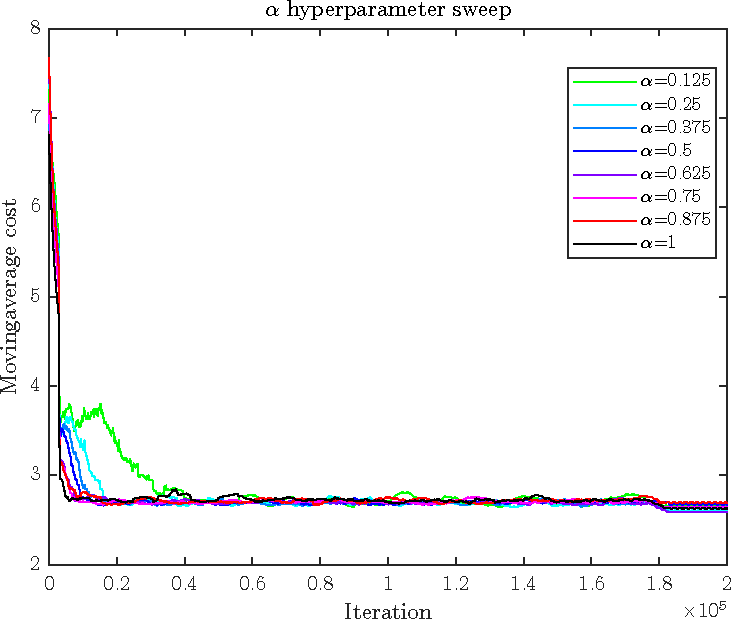
\includegraphics[width=0.7\linewidth]{figures/AlphaSweepTabRealHFull.pdf}
	\caption{Alpha sweep using 200000 iterations.}
	\label{fig:AlphaSweepTabularFull}
\end{figure} 

\begin{figure}
	\centering
	\begin{subfigure}{.5\textwidth}
		\centering
		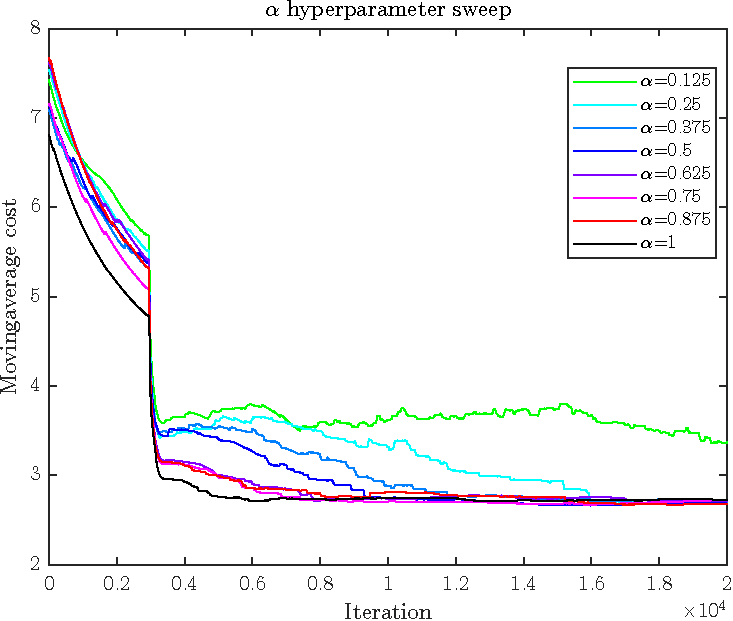
\includegraphics[width=1\linewidth]{figures/AlphaSweepTabRealHLeft.pdf}
		\caption{Initial convergence.}
		\label{fig:AlphaSweepTabularLeft}
	\end{subfigure}%
	\begin{subfigure}{.5\textwidth}
		\centering
		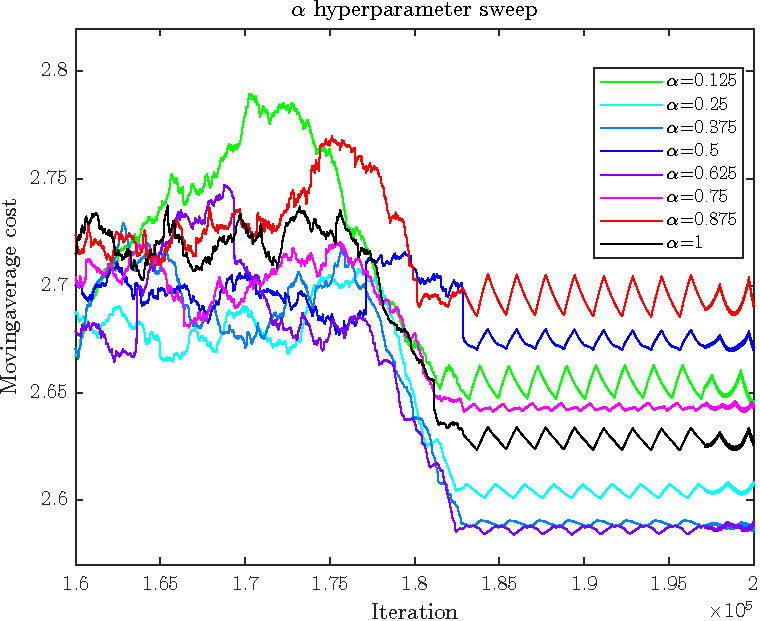
\includegraphics[width=1\linewidth]{figures/AlphaSweepTabRealHRight.pdf}
		\caption{Cutoff convergence.}
		\label{fig:AlphaSweepTabularRight}
	\end{subfigure}
	\caption{Zoomed images of left and right side of \cref{fig:AlphaSweepTabularFull} focusing on initial convergence and cutoff convergence.}
	\label{fig:Leftandright}
\end{figure}

\cref{fig:AlphaSweepTabularFull} shows how the moving average at different $\alpha$ values converge, see \cref{fig:Leftandright} for zoomed plots of beginning and end of the sweep. The long middle section for which it looks like all values have settled, is included to see if some values ultimately converge to a lower cost if it is allowed to see many random actions. The only clear tendency is that higher values converge faster.
In the final 10$\%$, no values appear better within the margin of randomness. Higher values are more susceptible to the random actions performed leading up to the cutoff, meaning there is a slightly larger spread of their final convergence cost.

\begin{figure}
	\centering
	\begin{subfigure}{.5\textwidth}
		\centering
		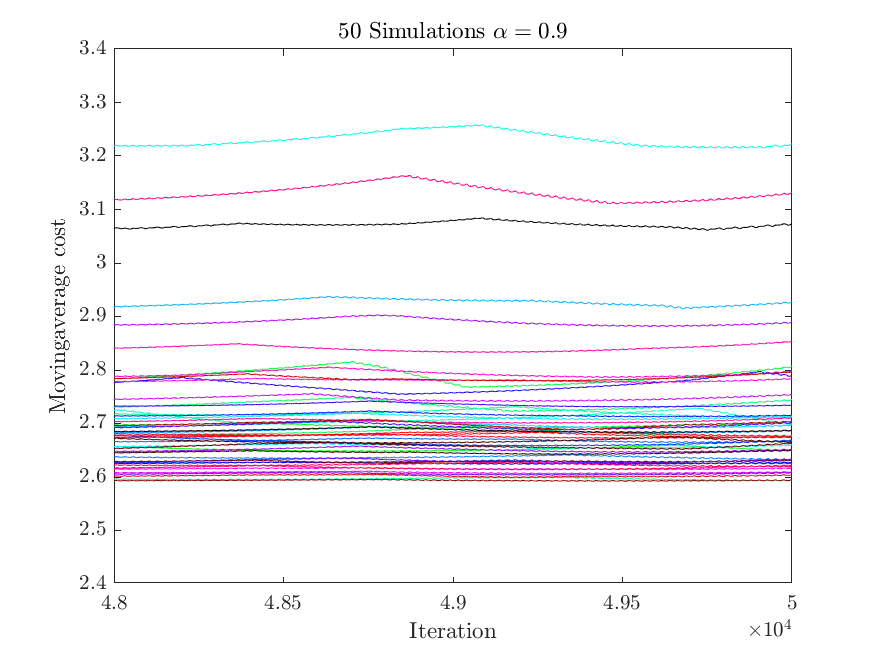
\includegraphics[width=1\linewidth]{figures/50plot09.pdf}
		\caption{Cutoff convergence of 50 simulations using $\alpha = 0.9$.}
		\label{fig:50plot09}
	\end{subfigure}%
	\begin{subfigure}{.5\textwidth}
		\centering
		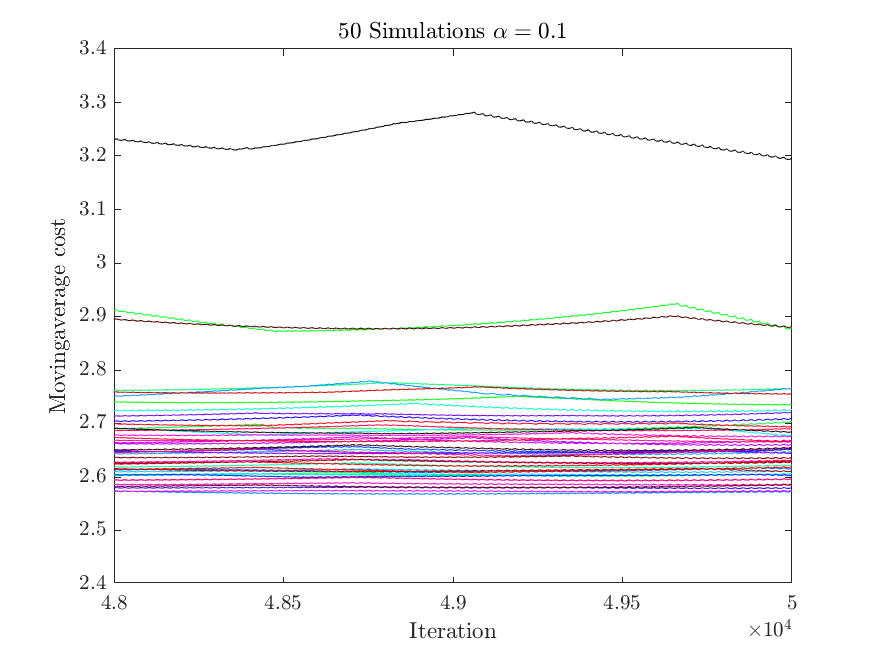
\includegraphics[width=1\linewidth]{figures/50plot01.pdf}
		\caption{Cutoff convergence of 50 simulations using $\alpha = 0.1$.}
		\label{fig:50plot01}
	\end{subfigure}
	\caption{Comparison of cutoff convergence of 50 simulations using $\alpha = 0.9$ and $\alpha = 0.1$. Notice colours do not carry meaning, as Matlab cannot distinguish 50 plots with different colours.}
	\label{fig:50plot}
\end{figure}

This tendency has been further explored by simulating values of $\alpha = 0,1$ and $\alpha = 0.9$ 50 times for 50000 iterations, see \cref{fig:50plot}. Higher values clearly show a higher variance. We also think the wider spread is due to higher $\alpha$ values \textit{bouncing} around the optimal minimum of the cost function. Similar to finding the minimum of a convex problem, a large step size will sometimes hit the minimum, but usually \textit{bounce} around in its vicinity.
Looking at the lowest and highest values, both seem to fluctuate more than the more moderate values in the middle part of \cref{fig:AlphaSweepTabularFull}, we suspect this is because the higher values over react, and the lower values are too slow to correct the influence of bad random actions.
We will select a value of $\alpha$ = 0.9, to gain fast initial convergence, and the downside of a wide spread is not big enough to merit a smaller value. 

A hypothesis on why such a large $\alpha$ is optimal is that there are no stochastic behaviour in this problem, any action at a certain state will always lead to a specific next state. As such, less filtering is needed, as the increment in action value is always in the direction toward the \textit{true} value.

The cutoff is presented as an aid in evaluation here, but could be implemented, while also gaining the benefit of a narrow spread, by reducing $\alpha$ to a much smaller value, either gradually or at some threshold e.g. after initial convergence.

\newpage \clearpage

\begin{figure}
	\centering
	\begin{subfigure}{.5\textwidth}
		\centering
		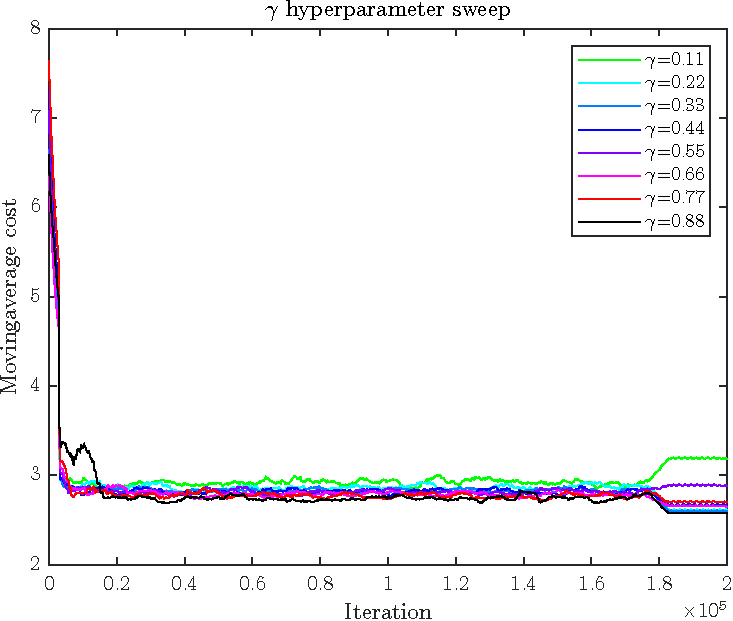
\includegraphics[width=1\linewidth]{figures/GammaSweepTabRealH.pdf}
		\caption{Gamma sweep full plot.}
		\label{fig:GammaSweepTabularFull}
	\end{subfigure}%
	\begin{subfigure}{.5\textwidth}
		\centering
		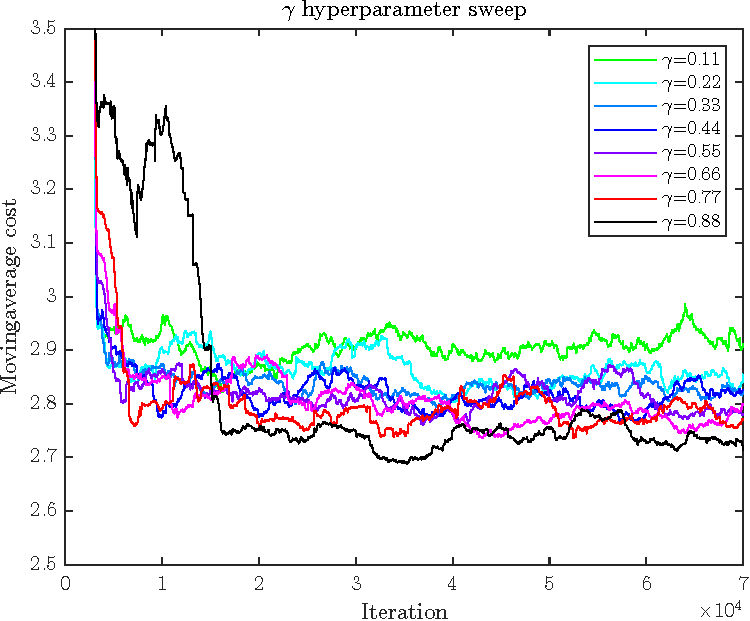
\includegraphics[width=1\linewidth]{figures/GammaSweepTabRealHZoom.pdf}
		\caption{Initial convergence.}
		\label{fig:GammaSweepTabularZoom}
	\end{subfigure}
	\caption{Gamma sweep showing the full plot (a), and a zoom focused on initial convergence (b).}
	\label{fig:Gammasweep}
\end{figure}

\cref{fig:Gammasweep} shows gamma sweep. There is also one clear tendency here, higher values converge slower, but settles lower once they have converged. The final moving average convergence value after the cutoff of all  $\gamma$ values fall within the margin of randomness, and therefore this area receives no further consideration.

\begin{figure}[h!]
	\centering
	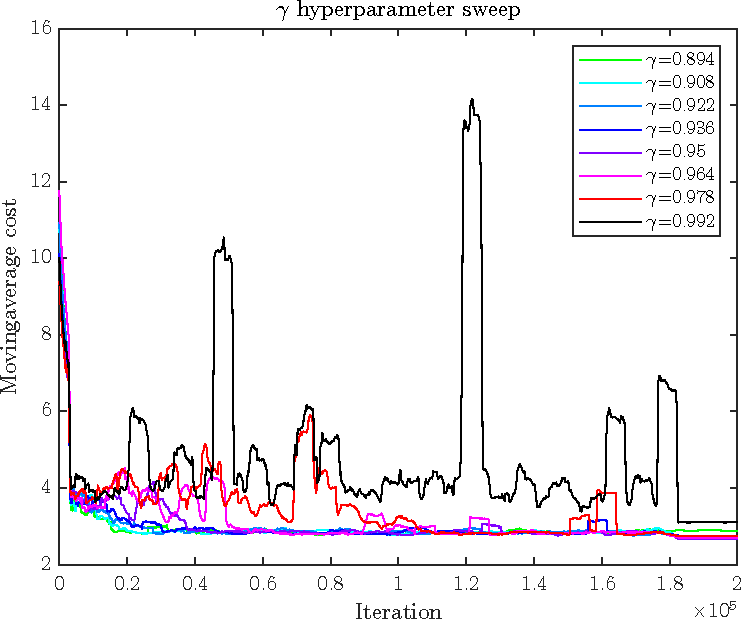
\includegraphics[width=0.7\linewidth]{figures/GammaSweepTabRealHNarrow.pdf}
	\caption{Additional narrow gamma sweep, including a finer sweep of high gamma values.}
	\label{fig:GammaSweepTabularNarrow}
\end{figure} 

\cref{fig:GammaSweepTabularNarrow} shows a narrow sweep of the very high values. A narrow sweep is performed for high values because the best value was expected to be in this range. Sweeps on previous iterations of the simulations scripts showed good performance with high $\gamma$, however, this is no longer valid. Higher values clearly slow convergence even further, to the point of not converging at all. Final convergence does not improve.
We choose a value of 0.77, since it is desired to converge as low as possible as fast as possible. Therefore we choose the highest values that does not increase convergence time a lot.

\begin{figure}[h!]
	\centering
	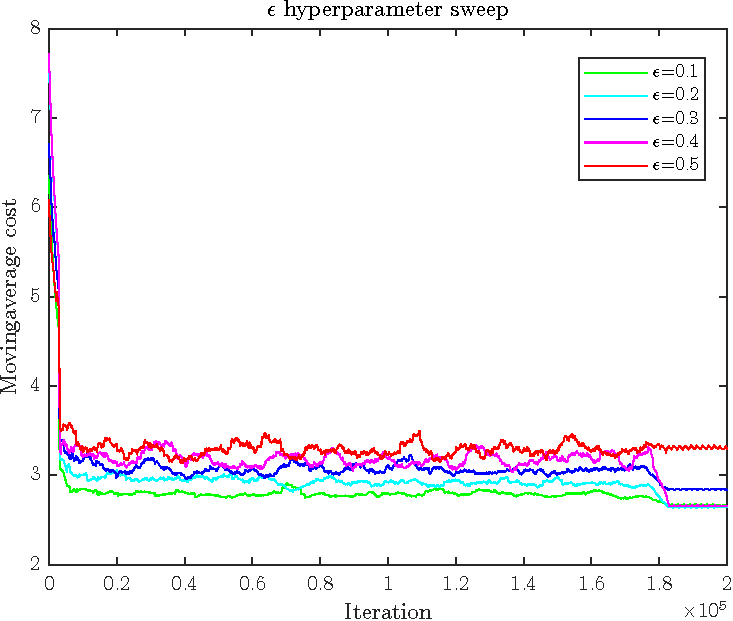
\includegraphics[width=0.7\linewidth]{figures/EpsilonSweepTabRealHWide.pdf}
	\caption{Epsilon sweep of relevant values between 0.1 and 0.5.}
	\label{fig:EpsilonSweepTabular}
\end{figure} 


\cref{fig:EpsilonSweepTabular} shows epsilon sweep for relevant values of $\epsilon$ ranging from 0.1 to 0.5, higher values means we are more random than not. A small $\epsilon$ standout as both yielding the smallest training cost, and lowest final convergence. This is expected from previous sweeps. Higher epsilon means the random influence leading up to the cutoff is greater\footnote{Remember we choose a quite high $\alpha = 0.9$.}, resulting in a greater spread of final convergence. Note $\epsilon = 0.1,0.4$ converge to similar final cost, showing that the high epsilon only increases the spread, not necessarily resulting in worse performance. The higher training cost is an obvious result of more random actions. We choose $\epsilon = 0.1$.

Final parameters are:
\begin{equation*}
	\alpha = 0.9 \hspace{1cm} \gamma = 0.77 \hspace{1cm} \epsilon = 0.1
\end{equation*}

  
\begin{figure}[h!]
	\centering
	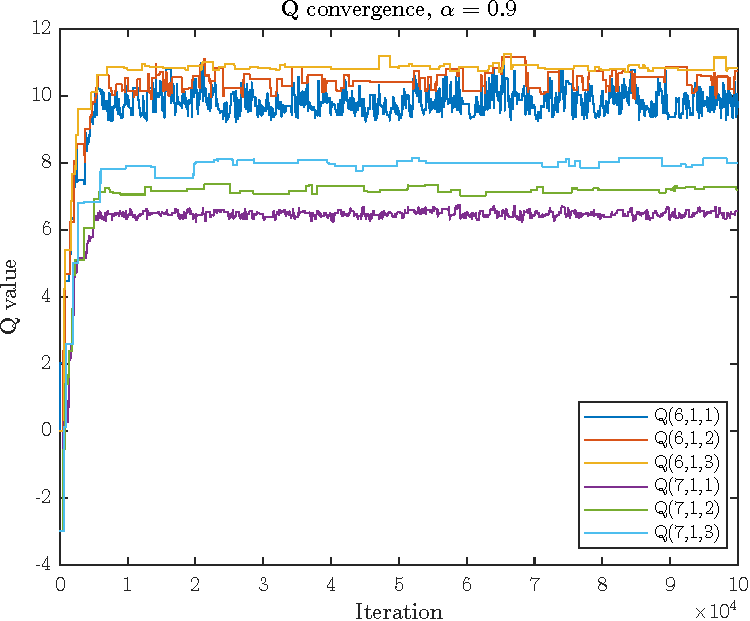
\includegraphics[width=0.7\linewidth]{figures/QConvergence09.pdf}
	\caption{Q convergence. Values for two different heights are shown, the lower height $h=7$, has an offset to add visual clarity to the plot.}
	\label{fig:Qconvergence09}
\end{figure} 

\begin{figure}[h!]
	\centering
	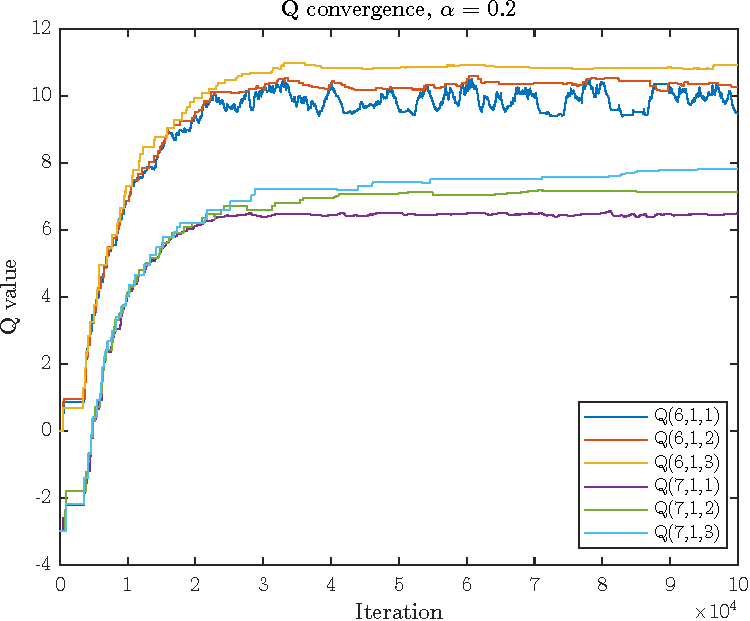
\includegraphics[width=0.7\linewidth]{figures/QConvergence02.pdf}
	\caption{Q convergence for reduced $\alpha$. Offset for visual clarity included again.}
	\label{fig:Qconvergence02}
\end{figure} 

As a few final remarks, we consider the convergence of the Q values, and with it an extra parameter evaluation on $\alpha = 0.2$ and $\alpha = 0.9$. The extra evaluation is included to present different water level behaviour, as seen in this paragraph. Q value convergence is a candidate for an alternative evaluation scheme instead of moving average cost for sweeps. \cref{fig:Qconvergence09} and \cref{fig:Qconvergence02} show Q convergence for $\alpha = 0,9$ and $\alpha = 0.2$ respectively. Notice that the \textit{chaoticness} of each signal is an indication of how often that specific state-action combination appears. Obviously the higher $\alpha$ value results in more oscillations, a lower value was included for comparison. Additionally, \cref{fig:QConvergenceBehavior} shows 5 simulations of reservoir water level plotted in the same plot. Here we see the impact of oscillations from high $\alpha$ are minor, the variance of the convergence of $\alpha = 0.2$ is smaller, but with more and greater outliers. Both share the same mean.

These results are more related to specific systems, and \textit{good} behaviour for that system. Sometimes less water level variance could be desired over fast convergence, therefore choosing a lower $\alpha$.

\begin{figure}
	\centering
	\begin{subfigure}{.5\textwidth}
		\centering
		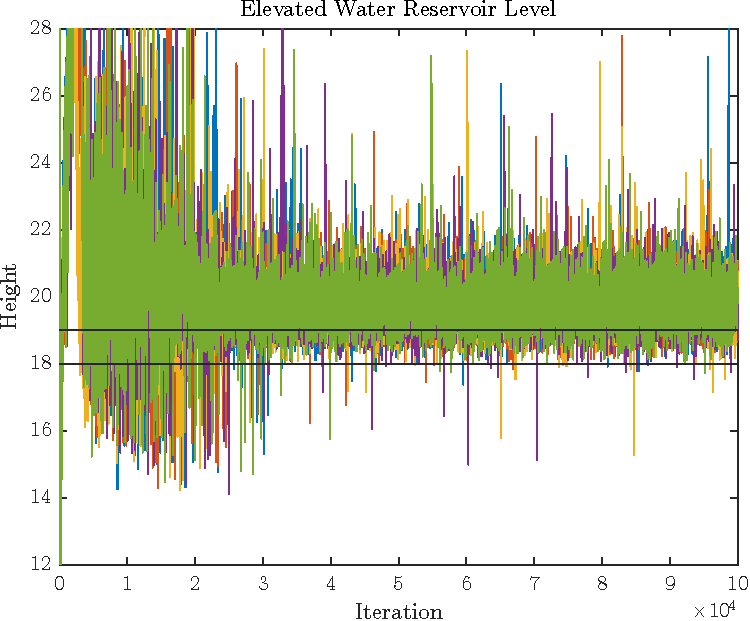
\includegraphics[width=1\linewidth]{figures/ConvergenceHeight02.pdf}
		\caption{5 simulations using $\alpha = 0.2$}
		\label{fig:5sims1}
	\end{subfigure}%
	\begin{subfigure}{.5\textwidth}
		\centering
		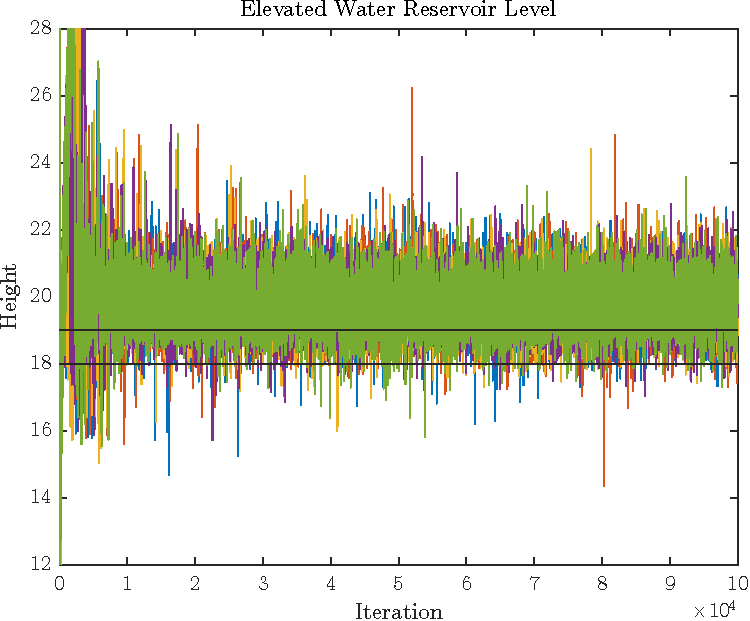
\includegraphics[width=1\linewidth]{figures/ConvergenceHeight09.pdf}
		\caption{5 simulations using $\alpha = 0.9$}
		\label{fig:5sims2}
	\end{subfigure}
	\caption{5 simulations in each plot used for comparison of high and low alpha, and the resulting behaviour of reservoir water level. Black lines are inserted at heights 18 and 19, to make differences more visible. Each colour is 1 of the 5 simulations.}
	\label{fig:QConvergenceBehavior}
\end{figure}

\newpage \clearpage

\subsection{Tabular Results}
Here we show simulation results using the swept parameters.

\begin{figure}[h!]
	\centering
	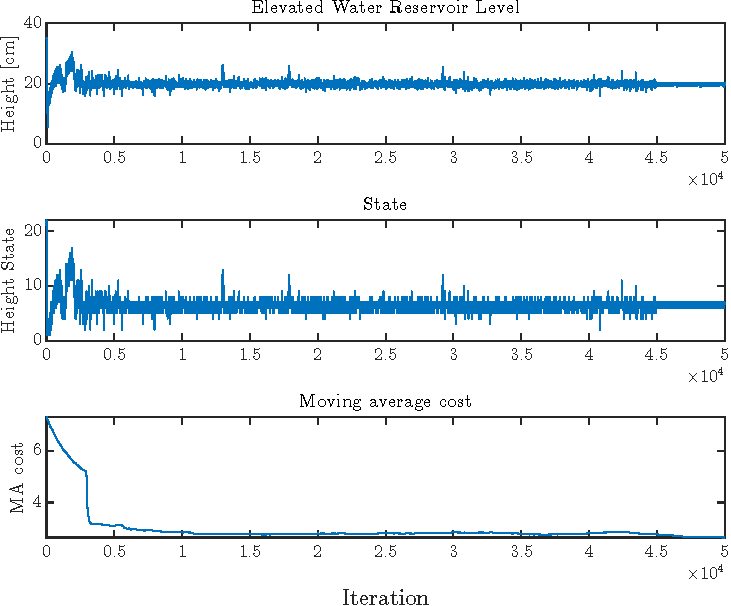
\includegraphics[width=0.7\linewidth]{figures/TabularResults2.pdf}
	\caption{Tabular Q learning results, showing elevated water reservoir level, state and moving average cost.}
	\label{fig:Tabularresults1}
\end{figure} 

\cref{fig:Tabularresults1} show reservoir water level, height state and the moving average cost. Water level converge nicely around the barrier at 20\si{cm}. The states are clearly explored from the bottom first, due to Matlab always choosing the first option when results of the \textit{minimum function} are equal, resulting in descending behaviour when initialising at 0. Let the term \textit{turnaround} denote to the ability to stop ascending-exploration of the height state, and begin to descend toward optimal values, before exploring the entire height space. This happens at iteration 1800 in \cref{fig:ResultRightZoom}. The \textit{turnaround} is unexpected, but results in much faster convergence as many states are unexplored. Some theories of why this happens is discussed in \cref{chap:Discussion}.

\begin{figure}[h!]
	\centering
	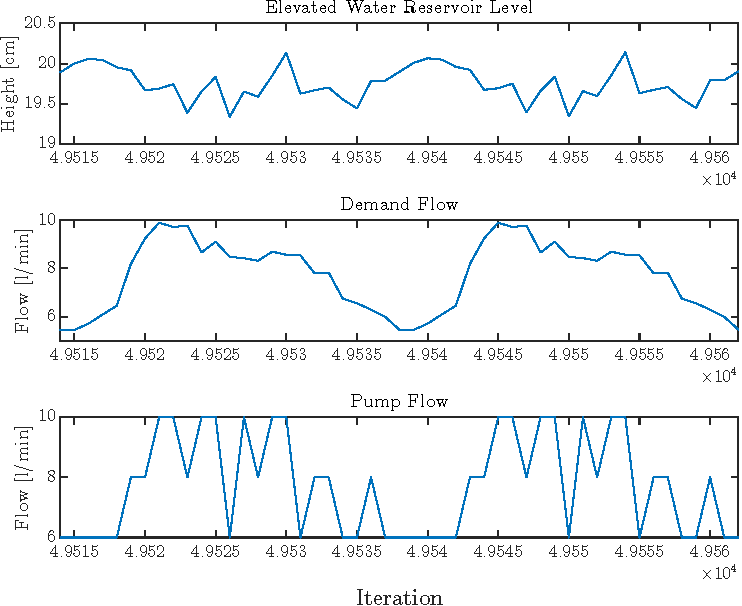
\includegraphics[width=0.7\linewidth]{figures/TabularResults1.pdf}
	\caption{48 hours tabular results,taken after the cutoff. Shows relationship between height, demand- and pump flow.}
	\label{fig:TabularResults2}
\end{figure} 

\cref{fig:TabularResults2} shows a 48 hour period after the cutoff. This clearly shows the dynamics between demand flow and pump flow (actions).

\begin{figure}
	\centering
	\begin{subfigure}{.5\textwidth}
		\centering
		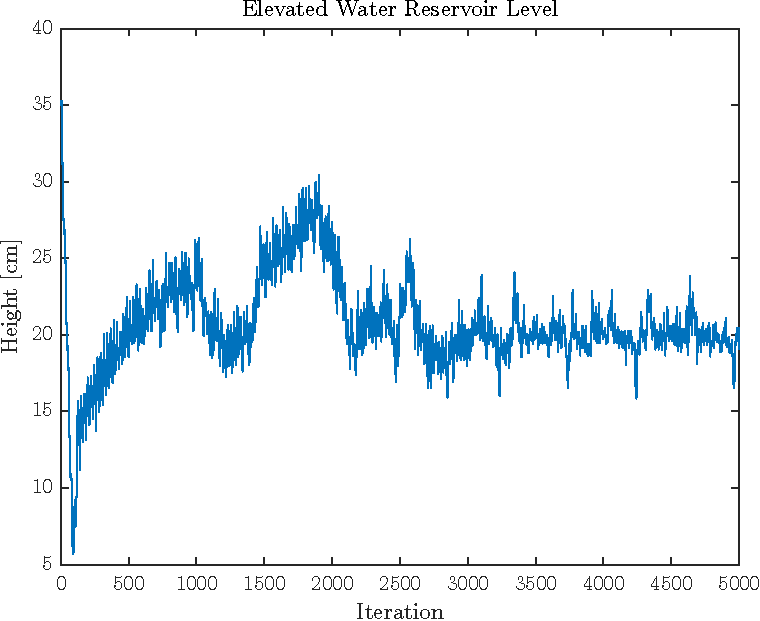
\includegraphics[width=1\linewidth]{figures/TabularResults3.pdf}
		\caption{Initial convergence.}
		\label{fig:ResultRightZoom}
	\end{subfigure}%
	\begin{subfigure}{.5\textwidth}
		\centering
		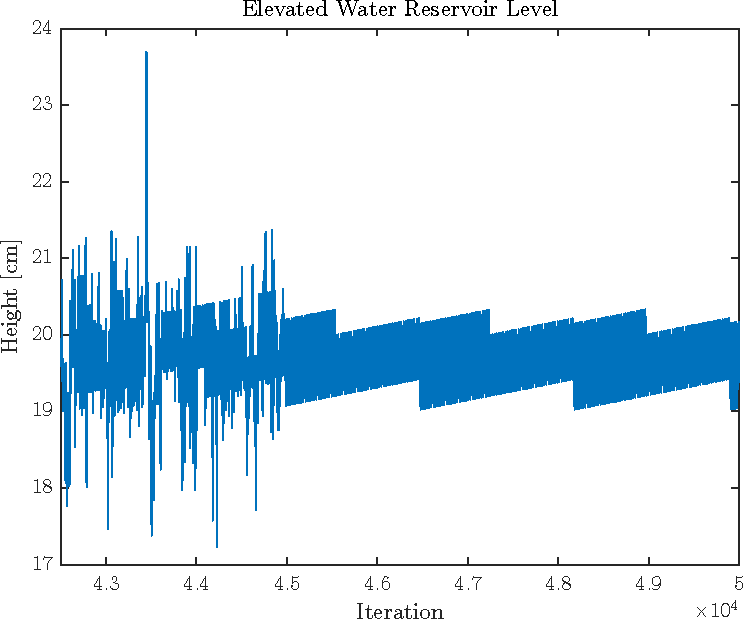
\includegraphics[width=1\linewidth]{figures/TabularResults4.pdf}
		\caption{Cutoff convergence.}
		\label{fig:ResultLeftZoom}
	\end{subfigure}
	\caption{Elevated water reservoir level results focused on initial convergence (a), and cutoff convergence (b).}
	\label{fig:ResultZoom}
\end{figure}

\cref{fig:ResultZoom} shows a zoomed image of the reservoir water level in the beginning and end of the simulation. In \cref{fig:ResultRightZoom}, notice the fast descend in the beginning (iteration 100), this is because action 1 is always chosen. Q is initialised to 0 for all state action pairs, and Matlab's min function always selects the first entry when min evaluations are equal. The rapid ascend back to 15, is because the state never changes, all states below 15 are set to state 1 due to height discretisation. Above the height of 15, dynamics slow down as new states are encountered at every height. 

The zigzag pattern in \cref{fig:ResultLeftZoom} is a result of slightly scewed demand balancing. The optimal policy simply results in a slight amount of excess water for every 24 hour period. If pumps or demand is altered slightly a smooth non-zigzag result can be obtained.

\clearpage \newpage

\section{Continuous Height, and Discrete Time and Action Q-Learning}\label{sec:sim1D}

As explained in \cref{sec:WDN1D} the action-value function can be approximated as:

\begin{equation}
	\hat{Q}\bigg(h(k),\textbf{w}_{t(k),a(k)}\bigg) =  \textbf{w}_{t(k),a(k)}\textbf{x}\bigg(h(k)\bigg)
\end{equation}

This section present simulation results obtained when applying continuous height, and discrete time and action Q-learning, to the water distribution in \cref{chap:WDN}. 

Weight vector is initialised to zero and updated according to \cref{alg:FuncApproxQ-learning} and radial basis functions are placed as explained in \cref{sec:WDNFunctionApproximationQ-Learning}. Hyper-parameter sweep is done similarly as in \cref{sec:TabularHSweep}, but plots are not shown, because tendencies cannot be seen in a single plot. Instead many simulations are done with varying combinations of hyper parameters, to build an intuition about system behaviour. The chosen parameters are:

\begin{equation*}
	\alpha = 0.4 \hspace{1cm} \gamma = 0.95 \hspace{1cm} \epsilon = 0.1
\end{equation*}

\begin{figure}[h!]
	\centering
	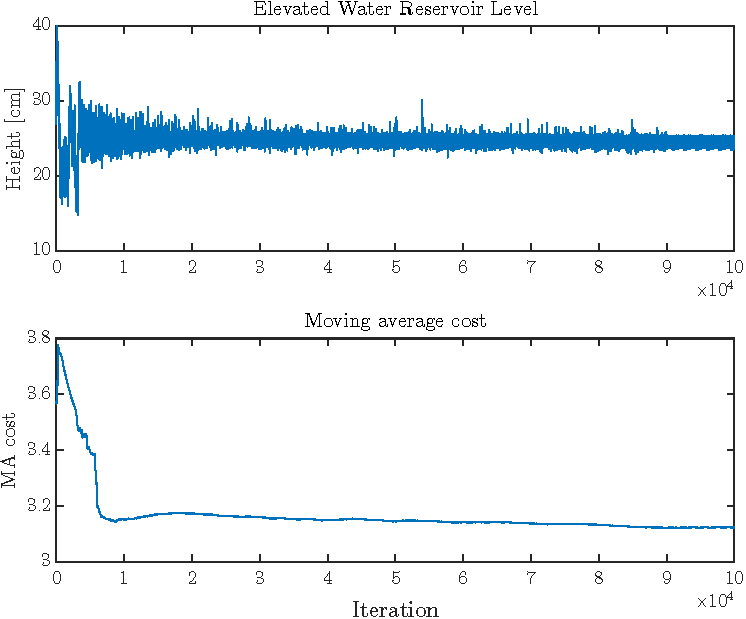
\includegraphics[width=0.7\linewidth]{figures/ContiniousHResults2.pdf}
	\caption{Continuous height approximation Q learning results. Showing elevated water reservoir level and moving average cost.}
	\label{fig:ContiniousHResults1}
\end{figure}

\cref{fig:ContiniousHResults1} presents water level in the elevated water reservoir and moving average of the cost function. Most noticeable is the tendency to settle much higher than the lower barrier, this is discussed further in \cref{chap:Discussion}. The benefit of generalisation is very apparent as the algorithm does not have to explore as aggressively to find the optimal policy.

\begin{figure}[h!]
	\centering
	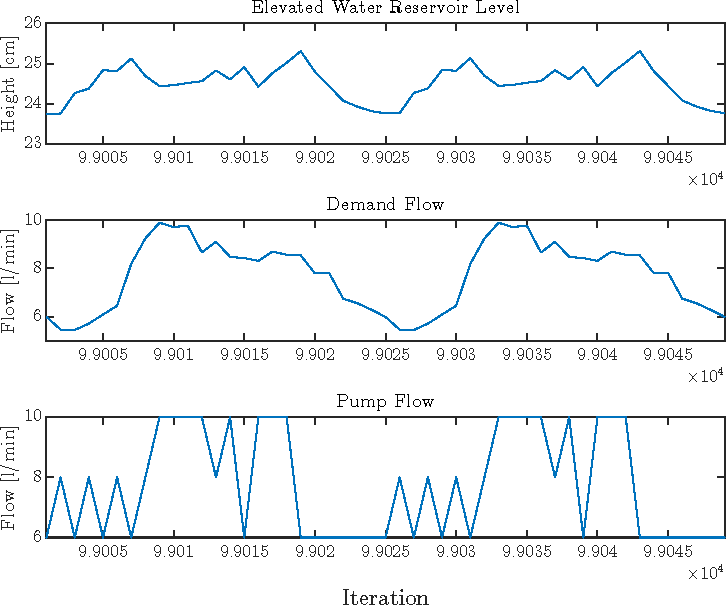
\includegraphics[width=0.7\linewidth]{figures/ContiniousHResults1.pdf}
	\caption{48 hours continuous height results, taken after cutoff. Shows relationship between height, demand- and pump flow.}
	\label{fig:ContiniousHResults2}
\end{figure} 

\cref{fig:ContiniousHResults2} shows a 48 hour period after the cutoff. It shows water levels similar to tabular method, pump flow (actions) are also similar, but clearly not the same. Although action value functions are obviously not exactly the same for both methods, this shows some proof of the concept that there exists several optimal policies (pump flows) which yield the same value function. 

\clearpage \newpage
\begin{figure}[h!]
	\centering
	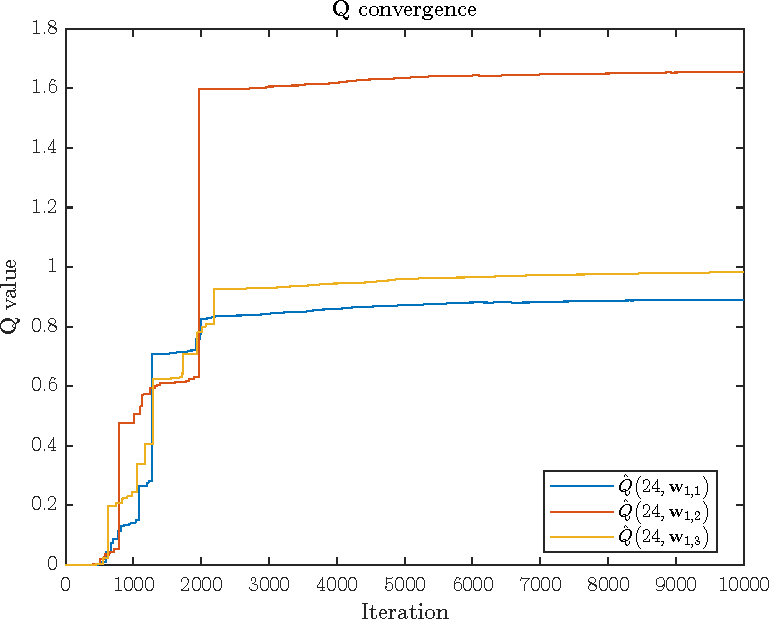
\includegraphics[width=0.7\linewidth]{figures/ContiniousHResults3.pdf}
	\caption{Q convergence for continuous height, at $h = 24,$ $t = 1$.}
	\label{fig:ContiniousHeightQConvergence}
\end{figure}
 
\cref{fig:ContiniousHeightQConvergence} presents convergence of approximated action value for height $ h=24\si{cm} $ and time $ t=1 $. Notice the x-axis is zoomed on iterations $0 - 10000$ to show the initial convergence. We can see the impact of generalisation by noticing that in the beginning (iteration 0 - 2000) of \cref{fig:ContiniousHResults1} the height is explored around $h=20$, however, \cref{fig:ContiniousHeightQConvergence} showing the Q value at $h=24$ shows changes at these iterations.


%Here we see some large jumps, even though the water level in the tank does not equal 24 at that time. These jumps happen when at $t = 1$ the specific action is made at some other water level. Due to generalisation, if that action yield a high cost, likely because the barrier is hit, there will be a large jump for all nearby heights.

\newpage

\iffalse
\subsection{Hyperparameters}
There are several hyperparameters which must be chosen, here we perform sweeps and evaluate performance to find a suitable hyperparameter value. Initial values are arbitrarily chosen, and each hyperparameter is then sequentially sweept. Initial values are shown below, parameters appear in the order they are swept:

\begin{equation*}
	\alpha = 0.1 \hspace{1cm} \gamma = 0.9 \hspace{1cm} \epsilon = 0.1
\end{equation*}

Sweeps are performed over singular parameters, ideally combinations of all parameters should be sweept, but we deem this too resource demanding. Performance is evaluated by looking at a moving average of the cost with a large window size, which helps smoothing out randomness. The final 10$\%$ of all simulations are without learning ($\alpha = 0$) or randomness ($\epsilon = 0$), this gives a more explicit indication of performance\footnote{E.g a large epsilon results in higher cost while learning, but lower cost after learning}. 

\begin{figure}[h!]
	\centering
	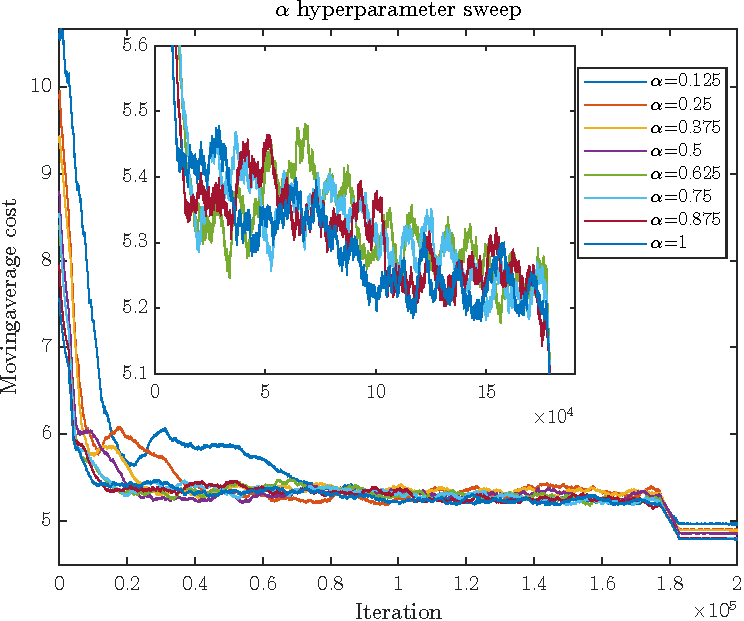
\includegraphics[width=0.7\linewidth]{figures/AlphaSweepApproxBest.pdf}
	\caption{Alpha sweep. Insert shows a zoomed image of the four largest alpha values.}
	\label{fig:AlphaSweep}
\end{figure} 

\cref{fig:AlphaSweep} shows different alpha values. Two tendencies are clear, larger alpha values both converge faster and to a lower cost. The insert shows a zoomed image of the four greatest alpha values. Here there are no clear discrephancies, and differences fall within the margin of randomness.

Simulations with $\alpha > 1$ shows cost diverging, although for $\alpha < 1.1$ cost sometimes converge as above. This correlate well with the properties in \cref{eq:alphaAssumptions}. We choose to use $\alpha = 0.75$ as this gives similar performance to higher values, and we assume higher values can cause problems if more weights are introduced.

\newpage
\clearpage

\begin{figure}[h!]
	\centering
	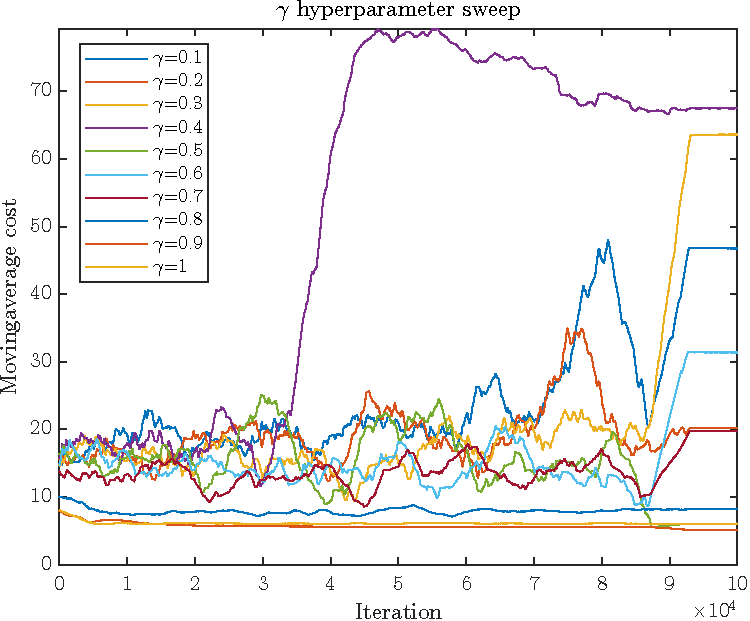
\includegraphics[width=0.7\linewidth]{figures/GammaSweepApproxWide.pdf}
	\caption{Wide gamma sweep. This is the first gamma sweep, sweeping over a wide range of values.}
	\label{fig:WideGammaSweep}
\end{figure} 

\cref{fig:WideGammaSweep} shows the first of two gamma sweeps. This is a wide sweep, considering a large range of values, this is done to identify where a narrow sweep should be performed. It is obvious that very high values yield best performance.

\begin{figure}[h!]
	\centering
	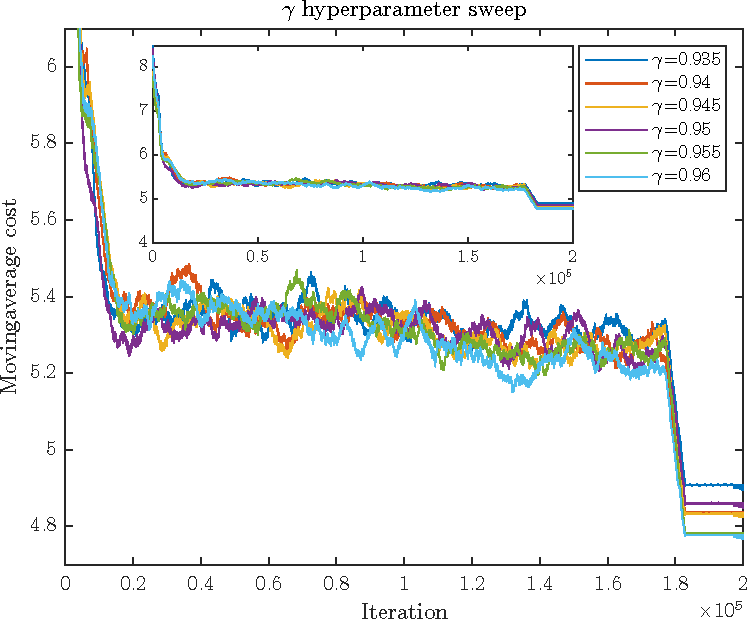
\includegraphics[width=0.7\linewidth]{figures/GammaSweepApproxNarrow.pdf}
	\caption{Narrow gamma sweep.}
	\label{fig:NarrowGammaSweep}
\end{figure} 

\cref{fig:NarrowGammaSweep} shows a narrow sweep at high values. Differences are susceptible to randomness, therefore multiple simulations of the above figure was performed, showing higher values consistently converge to a lower cost. \textit{We will see if even higher values are better, this plot lacks even higher values}.


\newpage
\clearpage
\begin{figure}[h!]
	\centering
	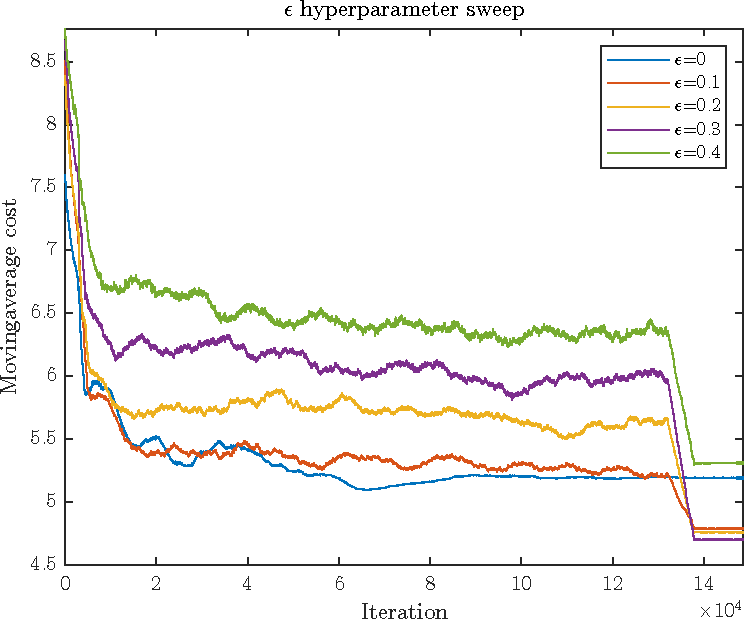
\includegraphics[width=0.7\linewidth]{figures/EpsilonSweepApprox.pdf}
	\caption{Epsilon sweep.}
	\label{fig:EpsilonSweep}
\end{figure} 

\cref{fig:EpsilonSweep} shows epsilon in the meaningful range between $0 < \epsilon < 0.5$, $\epsilon = 0$ is included for reference. At first glance the greedy algorithm without randomness looks decent, however, adding randomness leads to a lower convergence. More randomness seems to yield lower convergence up to a threshold. The highest epsilon (green), is worse than no randomness (blue), likely because the randomness explores actions in parts of the state space that are far from the optimal policy. There is simply not enough greediness to keep the algorithm in the area of the state space which contain the optimal policy, leading to pointless exploration.

A high epsilon leads to better performance after training, but at the sacrifice of performance while training, clearly shown by the layers in the figure. Therefore we choose $epsilon = 0.1$ to have the best performance while training, and still get the lower convergence that comes with exploration.
\fi


\clearpage
\newpage
\section{Continuous Level and Time, Discrete Action Q-Learning}


As explained in \cref{sec:WDN2D} The action value can be estimated using function approximation in both the height and time:

\begin{equation}
	\hat{Q}\bigg(h(k),t(k),\textbf{w}_{a(k)}\bigg) =  \textbf{w}_{a(k)}\textbf{x}\bigg(h(k),t(k)\bigg)
\end{equation}

Height approximation is done using weights and centers as previously. And time is approximated as presented in \cref{sec:WDN2D}. The weight vector is initialised and updated according to \cref{alg:ContFuncApproxQ-learning}. As previously, hyper parameter are swept but not shown. The following parameters are used:

\begin{equation*}
	\alpha = 0.2 \hspace{1cm} \gamma = 0.95 \hspace{1cm} \epsilon = 0
\end{equation*}

Notice $\epsilon = 0$, it was found that any randomness causes worse performance, and it is therefore not used. We present thought on \textit{implicit exploration} caused by Q initialisation and oscillating demand in \cref{chap:Discussion}.

\begin{figure}[h!]
	\centering
	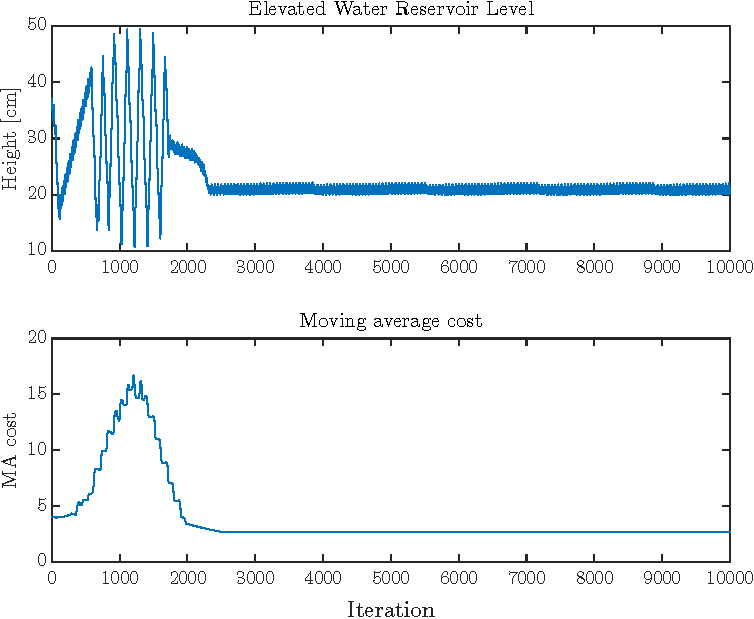
\includegraphics[width=0.7\linewidth]{figures/DoubleContResults1.pdf}
	\caption{Continuous height and time approximation Q learning results. Showing elevated water reservoir level and moving average cost.}
	\label{fig:DoubleContResults1}
\end{figure} 

\cref{fig:DoubleContResults1} presents water level in the elevated water reservoir and moving average of the cost function. Here we see a very defined initial learning, before converging to a final convergence value almost immediately. Notice that the final convergence is smoother than usual since $\epsilon = 0$. The first \textit{linear} learning explores the same state space as height approximation method, but then explores much broader. A very fast convergence around iteration 2200 is achieved, showing the power of generalisation. The final convergence value is also similar to that of the tabular method (better than height approximation). Notice the tendency to converge higher than the optimal value around $h_\star \approx 20$, which also was visible for height approximation, almost appears around iteration  2000. This tendency is even more apparent for different $\alpha$ values.

\begin{figure}[h!]
	\centering
	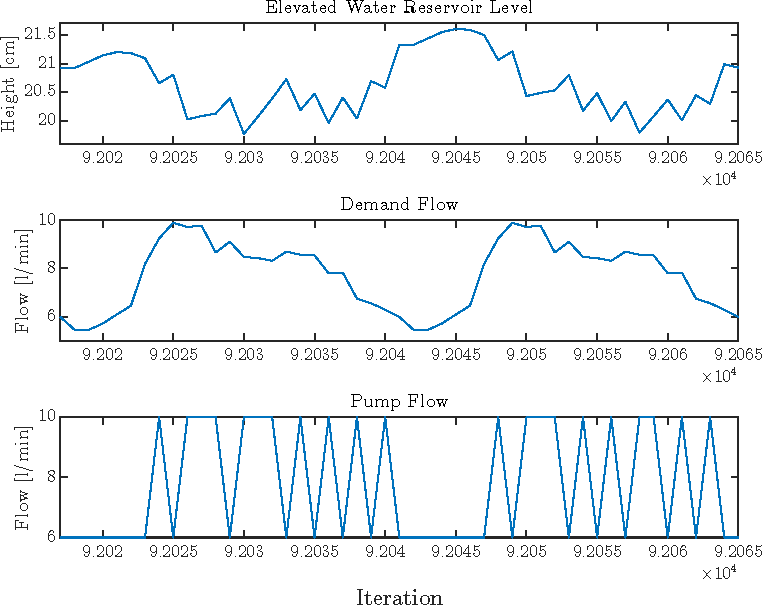
\includegraphics[width=0.7\linewidth]{figures/DoubleContResults2.pdf}
	\caption{48 hours continuous height and time results, taken after cutoff. Shows relationship between height, demand- and pump flow.}
	\label{fig:DoubleContResults2}
\end{figure} 

\cref{fig:DoubleContResults2} shows the same comparison as for the other methods. Notice there is no cutoff since this simulation does not include randomness. This means the pump profile is different for each 24 hour period, this tendency is also apparent if the cutoff is included, which would usually force equal action profiles for each 24 hour period. It seems generalising on time gives the algorithm more freedom, we do not grasp the full context to this \textit{feature}.

\begin{figure}
	\centering
	\begin{subfigure}{.5\textwidth}
		\centering
		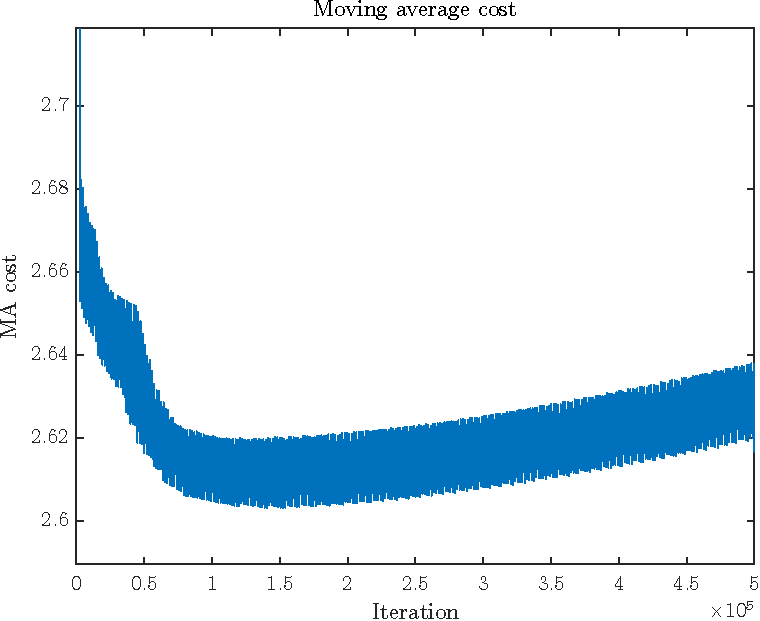
\includegraphics[width=1\linewidth]{figures/DoubleApprox02.pdf}
		\caption{Divergence of $\alpha = 0.2$.}
		\label{fig:Divergence02}
	\end{subfigure}%
	\begin{subfigure}{.5\textwidth}
		\centering
		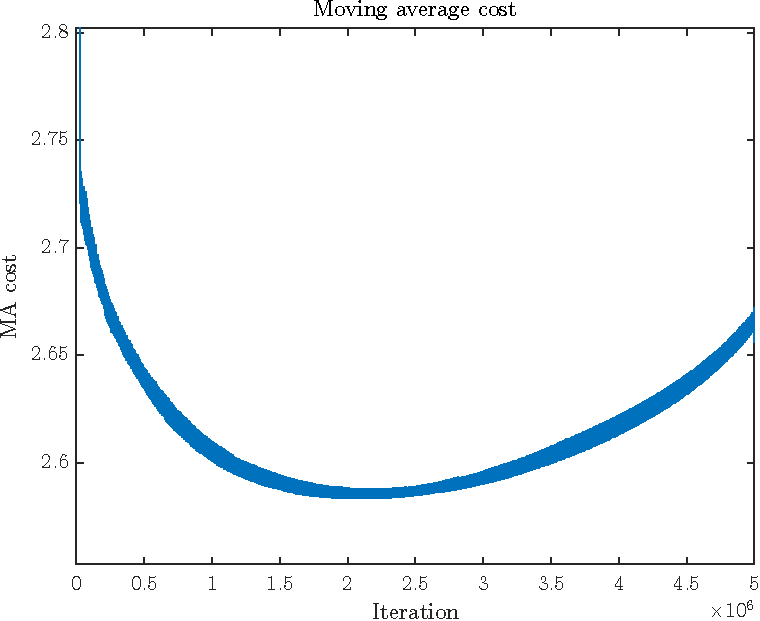
\includegraphics[width=1\linewidth]{figures/DoubleApprox001.pdf}
		\caption{Divergence of $\alpha = 0.01$.}
		\label{fig:Divergence001}
	\end{subfigure}
	\caption{Comparison of moving average cost beteween $\alpha = 0.2, \hspace{0.2cm} 0.01$.}
	\label{fig:DivergenceComparison}
\end{figure}

Although this method converges very fast, an issue is found if the simulation is extended. \cref{fig:DivergenceComparison} shows moving average costs for long simulations using $\alpha = 0.2\ \text{and}\ \alpha = 0.01$, both clearly diverge. We suspect this is caused by \textit{deadly triad} \cite{Sutton2020}. The deadly triad describes the danger of instability and divergence when combining the three following element: Function approximation, bootstrapping and off-policy training (Q-learning). On policy learning like \textit{SARSA} could be used to circumvent this issue.


\section{Method Comparison}

Function approximation has shown to be a very powerful tool, but also dangerous. Complexity increases drastically when approximating, intuition and knowledge about the algorithm's behaviour is much harder to obtain. We will make this comparison from the perspective of lab and real world implementation. In this context, double approximation is too parameter sensitive and likely to diverge, to be considered for real world implementation. The tabular method, showing similar convergence as height approximation, and even better final convergence, requires operation dangerously close to the  bottom of the tank. Height approximation show good performance and does not need to explore dangerous areas, therefore this method is the most suited for implementation at this stage of development. The performance of this method is further tested as it is applied to our water distribution network test setup in the following chapter.

\chapter{Laboratory Results}\label{chap:Results}
This chapter presents test results obtained when applying continuous height, discrete time and action function approximation Q-Learning to the Smart Water Infrastructure Laboratory shown in \cref{fig:AAUSWIL}, which is used to emulate the small scale water distribution network presented in \cref{sec:WDNsetup}.

Due to long convergence times the control method implemented is based on the final approximated action value function obtained in \cref{sec:sim1D}. This means control will be based on simulation learning, such that we do not have to learn in the laboratory. Because we have to wait for water level changes to happen, along with long convergence times at thousands of iterations, learning would take weeks in the real world. The performance results when using simulated training, depends on the similarities between test setup and simulations.

There are known differences between test setup and simulation, simulations use a model which is not entirely accurate to simulate water level changes. To reduce experiment length, an hour is made equivalent to one minute in the test setup. This gives behaviour similar to a changed flow or changed cross sectional area of the reservoir, meaning the change of water level will be different.

The test setup does not allow separate pumps to run independently. However, they do have speed control. Therefore rotational speeds will be set equally on two pumps at three different speeds, resembling three different actions. The speeds are chosen to yield combined flows matching simulation flows as well as possible.

Test details:
\begin{itemize}
	\item \textbf{Run time:} 144 minutes - representing 144 hours/6 days in real life. Simulations use time increments of one hour, we use the same concept for laboratory test, however, one hour will be equivalent to 1 minute. Among many things, this means a new actions is chosen every minute, and water level changes due to that actions, occur over the next 60 seconds.\\
	
	\item \textbf{Consumer demand:} Periodic over a 24 minute interval. 24 minutes (96 samples) represent 24 hours of a real day. Demand corresponds to normalised profile showed in \cref{sec:Consumption}. Demand is sampled every 15th second. Flows resembling simulation flows are obtained by controlling a variable valve with a PI-controller with the consumer profile described in \cref{sec:Consumption} used as a reference.\\
		
	\item \textbf{Time state:} As in simulation, time is discretises into 24 states \cref{sec:WDNTabularQ-Learning} and \cref{sec:WDN1D}.	
		
	\item \textbf{Weight vector \textbf{w}}: is obtained from simulation in \cref{sec:sim1D} and have dimension: $ \mathbb{R}^{3 \times 24 \times 10} $ corresponding to 10 radial basis functions with centers placement described in \cref{sec:WDN1D} \\ 
	
	\item \textbf{Actions:} are percentage pump rotational speeds, which are matched to fit simulation flows through trial and error before running results. As such actions are equivalent to rotational speeds of 50\%,\ 65\% and 100\%.
	
	\item  \textbf{Initial conditions:} initial water level of 38cm at $t=1$.
\end{itemize}

\begin{figure}[h!]
	\centering
	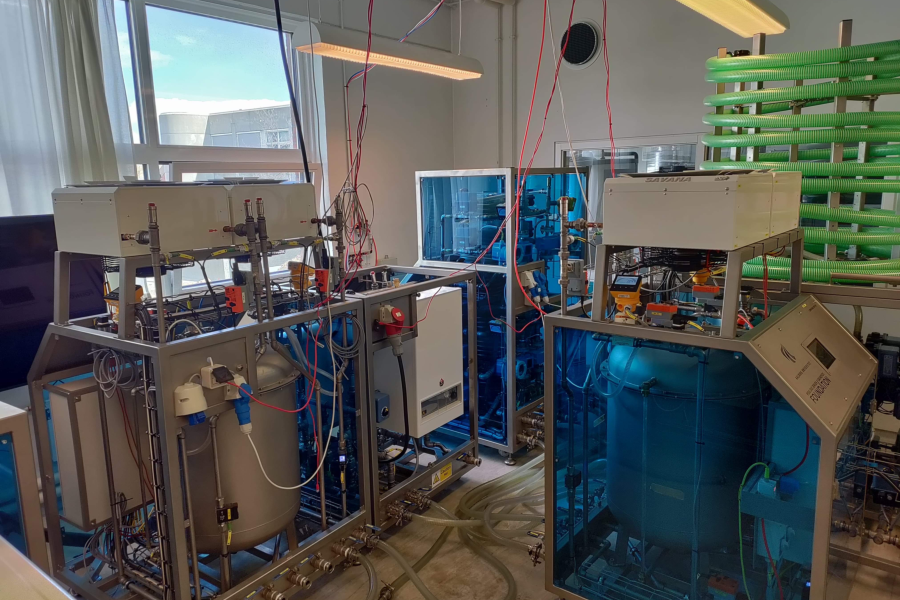
\includegraphics[width=0.7\linewidth]{Figures/SWIL.pdf}
	\caption{Picture of the AAU SWIL.}
	\label{fig:AAUSWIL}
\end{figure}

\clearpage

\section{Laboratory Setup}
\cref{fig:LabSetup} shows a diagram of the setup of laboratory modules. The pump station supplies water to the system, all water flows through a pipe module, both to add pipe length for a more realistic setup and to utilize the module's sensors. Water flows both to and from the elevated water reservoir. Flow to the consumer is regulated using a controllable valve in the module. Water is circulated using auxiliary pumps in the pump station. For a more detailed diagram of the setup, see Simulink setup in \cref{app:Simulink}. This diagram show simulink setup resembling the figure in this chapter, including specific names and numbers of the used sensors and  pumps.

\begin{figure}[h!]
	\centering
	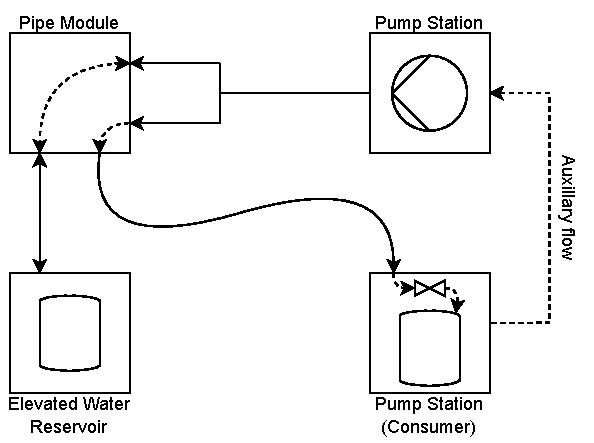
\includegraphics[width=0.7\linewidth]{Figures/LABsetupPDF.pdf}
	\caption{Diagram showing simple laboratory module setup.}
	\label{fig:LabSetup}
\end{figure}

\newpage

\section{Results}
\cref{fig:HtankResult} present the water level in the elevated water reservoir over a timespan of $ 144 $ minutes. Just like in \cref{chap:Simulation} a periodicity is visible in the water level, which is expected due to the periodicity in the consumer demand shown in \cref{fig:Consumption}. Water level is nicely reduced to the optimal value around 25 as expected similarly to simulation results in \cref{sec:sim1D}. The fact that the water level settles so far above the barrier in both simulation and laboratory is discussed in the following chapter. 

The simulated mean water level for the last five periods is $24.55$ and for laboratory results the mean is $25.25$, which we consider to be similar behaviour. The water level variance seems greater for laboratory results, likely because the demand is sampled four times more often, and demands are not as accurate as in simulation, since the demand is controlled via a valve which has a settling time.

\begin{figure}[h!]
	\centering
	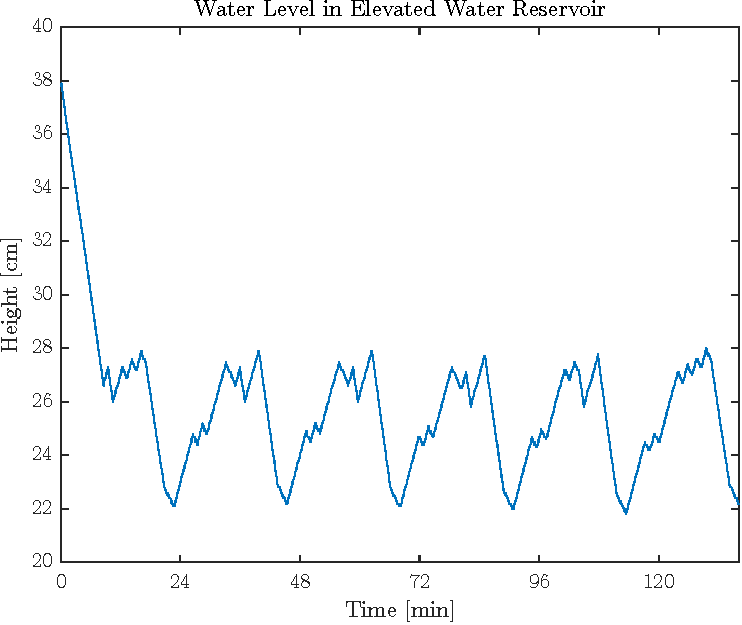
\includegraphics[width=0.7\linewidth]{figures/ResultHeight.pdf}
	\caption{Water level in elevated water reservoir, showing a period of 5 days.}
	\label{fig:HtankResult}
\end{figure}

The difference to simulation results was expected based on the already known differences between test setup and simulation. One of the advantages to reinforcement learning mentioned in this project is its ability to adapt to changes in the environment. However, this implementation does not include learning, due to Simulink implications. We are certain that a full reinforcement learning method with learning and exploration can be implemented in Simulink, but was not within scope of this project.

Furthermore, for the same reasons, this implementation does not include exploration. The nature of the Simulink issues are from storing previous values while the simulation is running. We do not see any reason that this should not be doable in Simulink if more time was available. 

\cref{fig:PumpResult} shows actions chosen by the reinforcement learning agent. A  periodic pump profile is visible as expected. Notice the lowest rotational speed is used as long as there is too much water in the reservoir.

\begin{figure}[h!]
	\centering
	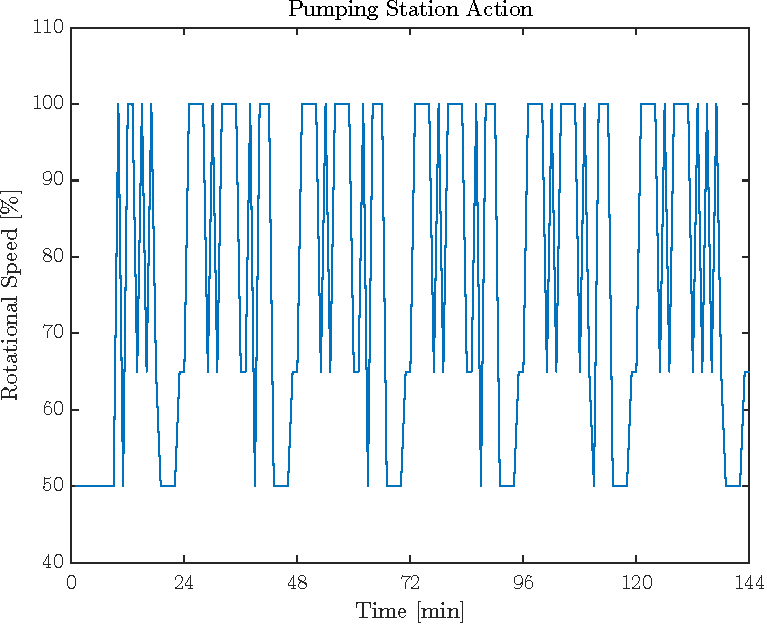
\includegraphics[width=0.7\linewidth]{figures/ResultPumpSpeed.pdf}
	\caption{Pump profile showing rotational speed (actions) over time.}
	\label{fig:PumpResult}
\end{figure}



\chapter{Discussion}\label{chap:Discussion}

This section presents a discussion related to results throughout this project. We present hypothesis and thoughts on different aspects of results. 

\section{Demand Balancing}

Due to the limited number of action the demand has to be matched to fit the pump flows. If this matching is not done nearly perfect results are diverging. An unbalanced demand, means large periods of the demand are greater or smaller than the highest or lowest pump flow respectively. Without randomness reinforcement learning handles the imbalance, it essentially requires that you always follow the best actions. Without grasping the full context or reasoning to this problem, randomness sometimes results in an action which starts a loop of bad actions, resulting in divergence. From many hours of simulation, heuristic evidence, show balancing demands make the algorithm much more robust toward randomness.

In the results shown in \cref{chap:Simulation} and \cref{chap:Results} the pump flow are:

\begin{equation*}
q(k)=\{6\;\; 8 \;\; 10\}l/min
\end{equation*}

and the demand flows are:

\begin{equation*}
	d(k)\in [5.44,\; 9.9] \; l/min
\end{equation*}


 A potential solution could be to add more pumps to the pumping station, which would result in more actions and a better coverage of varying demand profiles. This in turn increases the size of the table in tabular Q-learning and adds extra weight vectors in function approximation Q-learning with discrete actions. 
With perspective to the real world, where additional pumps come at a cost, and demands cannot be controlled. The option of running 0 pumps should be included and pumps should be slightly too powerful equivalent to demands being balanced slightly too low.

\section{Hyperparameters}
As mentioned previously sweeping hyperparameters sequentially is not ideal. In future work these sweeps should be performed more thoroughly by evaluating combinations of parameters. Any change of one hyperparameter changes the optimal selection of the other parameters. This could not be done within the scope of this project, due to coding- and simulation time required to obtain the results. 

The \textit{tendencies} that are often refereed to in sweeping results are subject to randomness, especially for the height approximation method. In reference to the \textit{law of large numbers} tendencies would require a large amount of simulation before being applicable. Results in this project are simulated multiple times, but not enough. This induces some ambiguity in the results of the sweeps. In future work, the ideal sweep incorporates both combinations of parameters and satisfy the law of large numbers.

In a thorough sweep we also suggest considering the convergence of Q values as an evaluation metric. We have not used this method enough to express its advantages, but there seem to be useful information to be achieved in addition to moving average cost evaluation.

Finally a few thoughts on the \textit{cutoff} and its implementation. The cutoff was used in this project as an evaluation tool, but could be implemented by reducing $\epsilon$ and $\alpha$ either after a iteration threshold or continuously. This would unlock the optimal behaviour, instead of adding some suboptimal behaviour from learning and exploration. If changes to the environment are expected, these parameters could be increased to detect and learn these changes, and then reduced back to cutoff values, continuing optimal behaviour.

\section{Premature Convergence}
The tabular method shows the ability to converge without exploring the entire state space. This is against expectations, but we present a two part explanation. First we place emphasis on the oscillating demand, which allows the algorithm to see a specific state multiple times without knowing how to \textit{stay} in that state. Secondly each time a state is seen, the algorithm gets one step closer to learn the optimal action in that step. We will consider the scenario where ascending states are explored, heading toward the top of the reservoir. As we explore the \textit{0 cost} area of the barrier function, the only cost assigned to a state is primarily from the action (flow) itself, and the pressure induced from reservoir water level \ref{eq:WDN_Power}. As the tank level rise, the increments of the action cost increases, and these increments increase a lot more when the barrier is hit. When the difference in increments are big enough, the algorithm will choose the lower action increasingly many times in a row before the cost has incremented far enough that its cost is higher than another action's. Eventually, the number of \textit{low-flow} actions in a row, will result in the water level decreasing further than what is expected from the demand at that time. This unexpected decrease results in the algorithm seeing a state that it has already fully learned, and it will deliberately select the optimal action and end the upward exploration. From here on, the algorithm descends down without any reason to go back up.

We assume this theory also applies to the height function approximation method's ability to just barely explore the upper barrier. 


\section{Extending Radial Basis Center Placement}
To give the best initial conditions without prior knowledge, the sum of radial basis function should equal 1. If centers are placed at the edges of the range, the sum near the edges will be less than 1, meaning lower emphasis is put on the very edges, this is intuitively not a smart starting point for learning. Edges could be argued to be the most important and interesting areas. Therefore centers where tried extended outside the range, resulting in a similar sum over the entire range. 

This was thought to increase performance for all algorithms, although we now believe the increased performance was from more favourable placement of all centers, which happened indirectly when extending the centers on the edge to maintain uniform placement.

The context to extending centers could not be examined sufficiently within the scope of this report, and we would like to research this topic further in future work.

\newpage

\section{Barrier Overflow}
Height approximation results settle much higher than tabular method, this is because generalisation from radial basis functions extends the cost of the barrier further than its beginning. The entire middle part of the barrier gives 0 cost, but with generalisation the cost of entering the barrier will overflow into the heights that should otherwise belong to the \textit{0 cost area} of the barrier. \cref{fig:RBFandBarrier} shows the radial basis function with center nearest the barrier beginning.

\begin{figure}[h!]
	\centering
	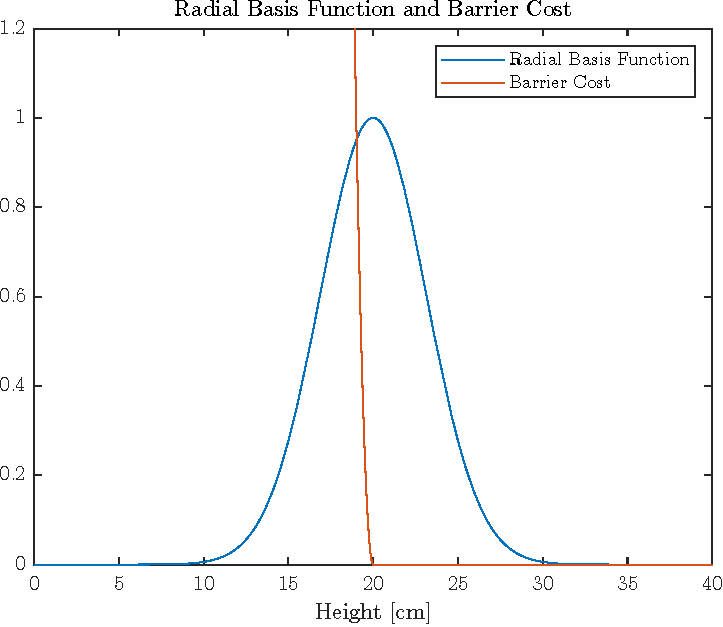
\includegraphics[width=0.7\linewidth]{figures/RBFandBarrier.pdf}
	\caption{Beginning of barrier and radial basis function with center closest to barrier beginning.}
	\label{fig:RBFandBarrier}
\end{figure}


\begin{figure}[h!]
	\centering
	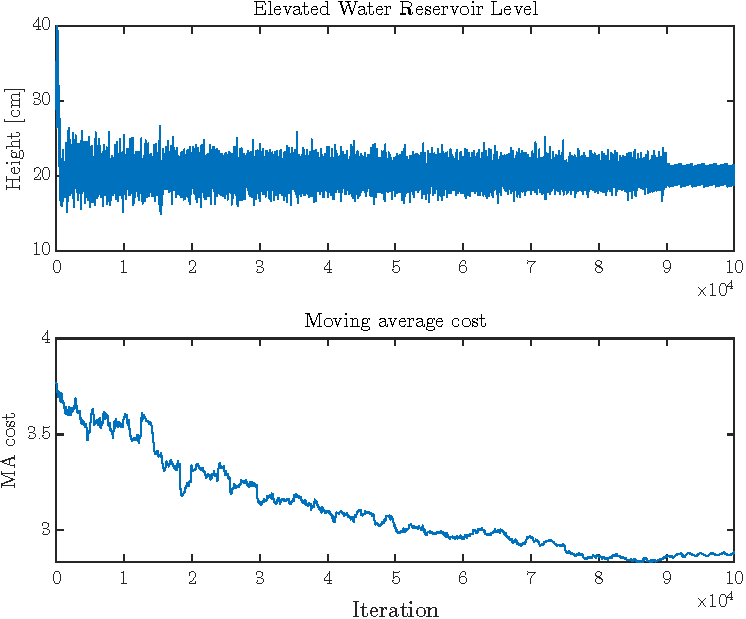
\includegraphics[width=0.65\linewidth]{figures/RemovedCenter.pdf}
	\caption{Continuous height results with feature near lower barrier removed.}
	\label{fig:RemovedCenter}
\end{figure}

\cref{fig:RemovedCenter} shows the results of removing the feature with center near the beginning of the lower barrier. The initial convergence now reaches much closer to the expected optimal height, but convergence in that area is much slower. Because points here are far away from any feature, their impact are weighted very low.

\begin{figure}[h!]
	\centering
	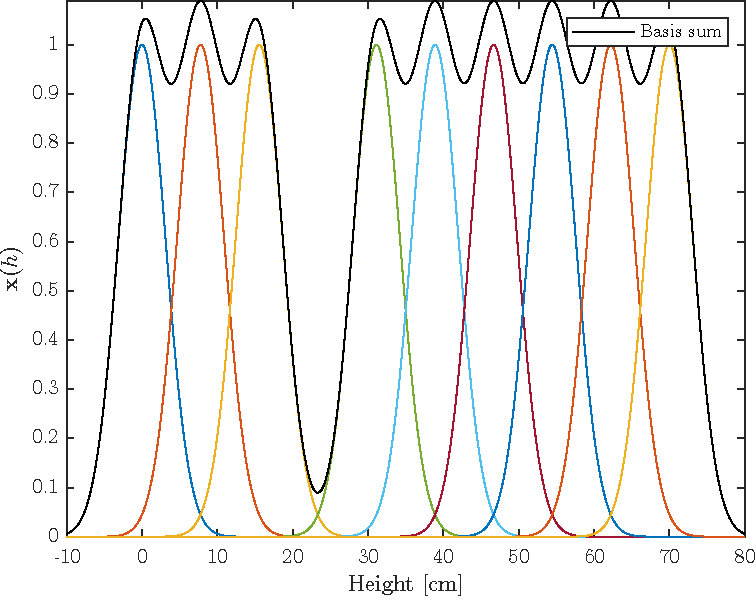
\includegraphics[width=0.65\linewidth]{figures/RemovedRBF.pdf}
	\caption{Radial basis functions with center near barrier removed.}
	\label{fig:RemovedRBF}
\end{figure}

\cref{fig:RemovedRBF} shows the radial basis functions with the center closets to barrier beginning removed. This clearly visualises the reason that overflow is reduced, but at the expense of having very little feature impact in that area causing learning to be very slow.

Another approach to removing the center, is to add more narrow radial basis functions around the barrier beginning. This would cause the generalisation to be more accurate, meaning less overflow, without sacrificing learning.

Essentially, the number of radial basis functions, and placement of their centers can and should be included as a hyperparameter.


\section{Implicit Exploration}
full state function approximation results showed seemingly very nice convergence without randomness, although it ultimately diverges. This initial nice behaviour, even without randomness is possible because of implicit exploration from other elements. The oscillating demand very clearly results in a similar oscillation in state, this is seen in all water level plots. Initialisation of Q values and weights at 0, means whenever a cost is assigned to one action, all other actions are better until they have shown to yield even higher cost. The combination of these is very clear in the full state function approximation results \cref{fig:DoubleContResults1}, showing a very large range of states being explored before convergence.

\section{Generalisation to other Water Distribution Networks and Real World Implementation}
this section presents thoughts on the real life implementation of reinforcement learning. We have seen all method be quite sensitive to hyperparameters, and performance relies on demand balancing. We therefore doubt the method is easily applicable to all networks, some redesign and tuning will certainly be necessary. However, the laboratory results are performed without a finely tuned algorithm, and shows that decent performance can be achieved with direct implementation. Finally, the tuning of a reinforcement learning algorithm is likely much less tedious than modelling a complete water distribution network, if it is even possible.

We have mentioned the minimisation of energy as a goal of this project. We cannot present evidence of this goal, but believe there is good reasoning to believe reinforcement learning can reduce energy usage. The algorithm clearly settles to a optimal behaviour in regards to the formulated cost function. Whether this is actually optimal would require modelling of the system, and heavily depend on design of cost function and barriers. There is also the element of safe learning, the act of learning, without imposing dangerous states on the system. In this project the only indirect safety feature is imposed by the barrier function. Here we see the trade off between optimality and safety,  where the beginning of the lower barrier determines how low the algorithm settles, directly influencing the energy needed to satisfy demands.

Although approximation methods are showing safe learning, due to generalisation. We would not guarantee safe behaviour from these methods, before real implementation, methods to guarantee safe learning needs to be found. Further more, we remark the importance of demand balancing, which in real implementation can only realistically be done by carefully designing the pump setup, as demands cannot be controlled. 


\chapter{Conclusion}\label{chap:Conclusion}
As suggested in \cref{sec:projectDescription} the objective of this project was design and implementation of a optimal and model free  controller for a water distribution network. Three reinforcement learning methods have been applied and compared; tabular Q-learning, continuous height, and discrete time and action function approximation Q-learning, and continuous height and time, and discrete actions function approximation Q-learning. When comparing these three methods it was found that the best control method for real life implementation was continuous height, and discrete time and action function approximation Q-learning due to its ability to generalise, giving better behaviour than the tabular method. The method is also superior to continuous height and time, discrete actions function approximation Q-learning, since this method shows unpredictable and diverging results, and also seems so be extremely hyperparameter sensitive compared to the two other methods. Even though we observe diverging result the method is an interesting candidate for further work since simulations show superior initial performance when comparing moving averages of the cost function. 

Although the examined methods are not compared to existing water distribution network control methods, relative to pumping station energy consumption, we feel confident in saying that the formulated cost function ultimately guarantees minimal energy consumption.

Laboratory testing indicates that continuous height, and discrete time and action function approximation Q-learning is a viable control method that works well, when training is done in a simulated environment. Training in a real life environment was not within the scope of the project, but the implementation lays the foundation for future work and has given us a strong belief that reinforcement learning methods are well suited for real life implementation and can make a difference on both existing and new systems. We note that reinforcement learning control methods developed should include some kind of safety aspect such that safety constraints of systems are not violated. 


%\input{sections/futurework.tex}
\printbibliography[heading=bibintoc]
\label{bib:mybiblio}

\clearpage
\appendix

\chapter{Continuous height discrete time and action Q-Learning MATLAB Script} 

\section{New state script}

\lstinputlisting[caption = {New state and action script}]{code/nextstatefunctionapprox.m}

\clearpage \newpage
\section{Weight update MATLAB script}

\lstinputlisting[caption = {Weight update script}]{code/continuousHeight.m}

\clearpage \newpage
\section{Simulink setup}\label{app:Simulink}
\begin{figure}[h!]
	\centering
	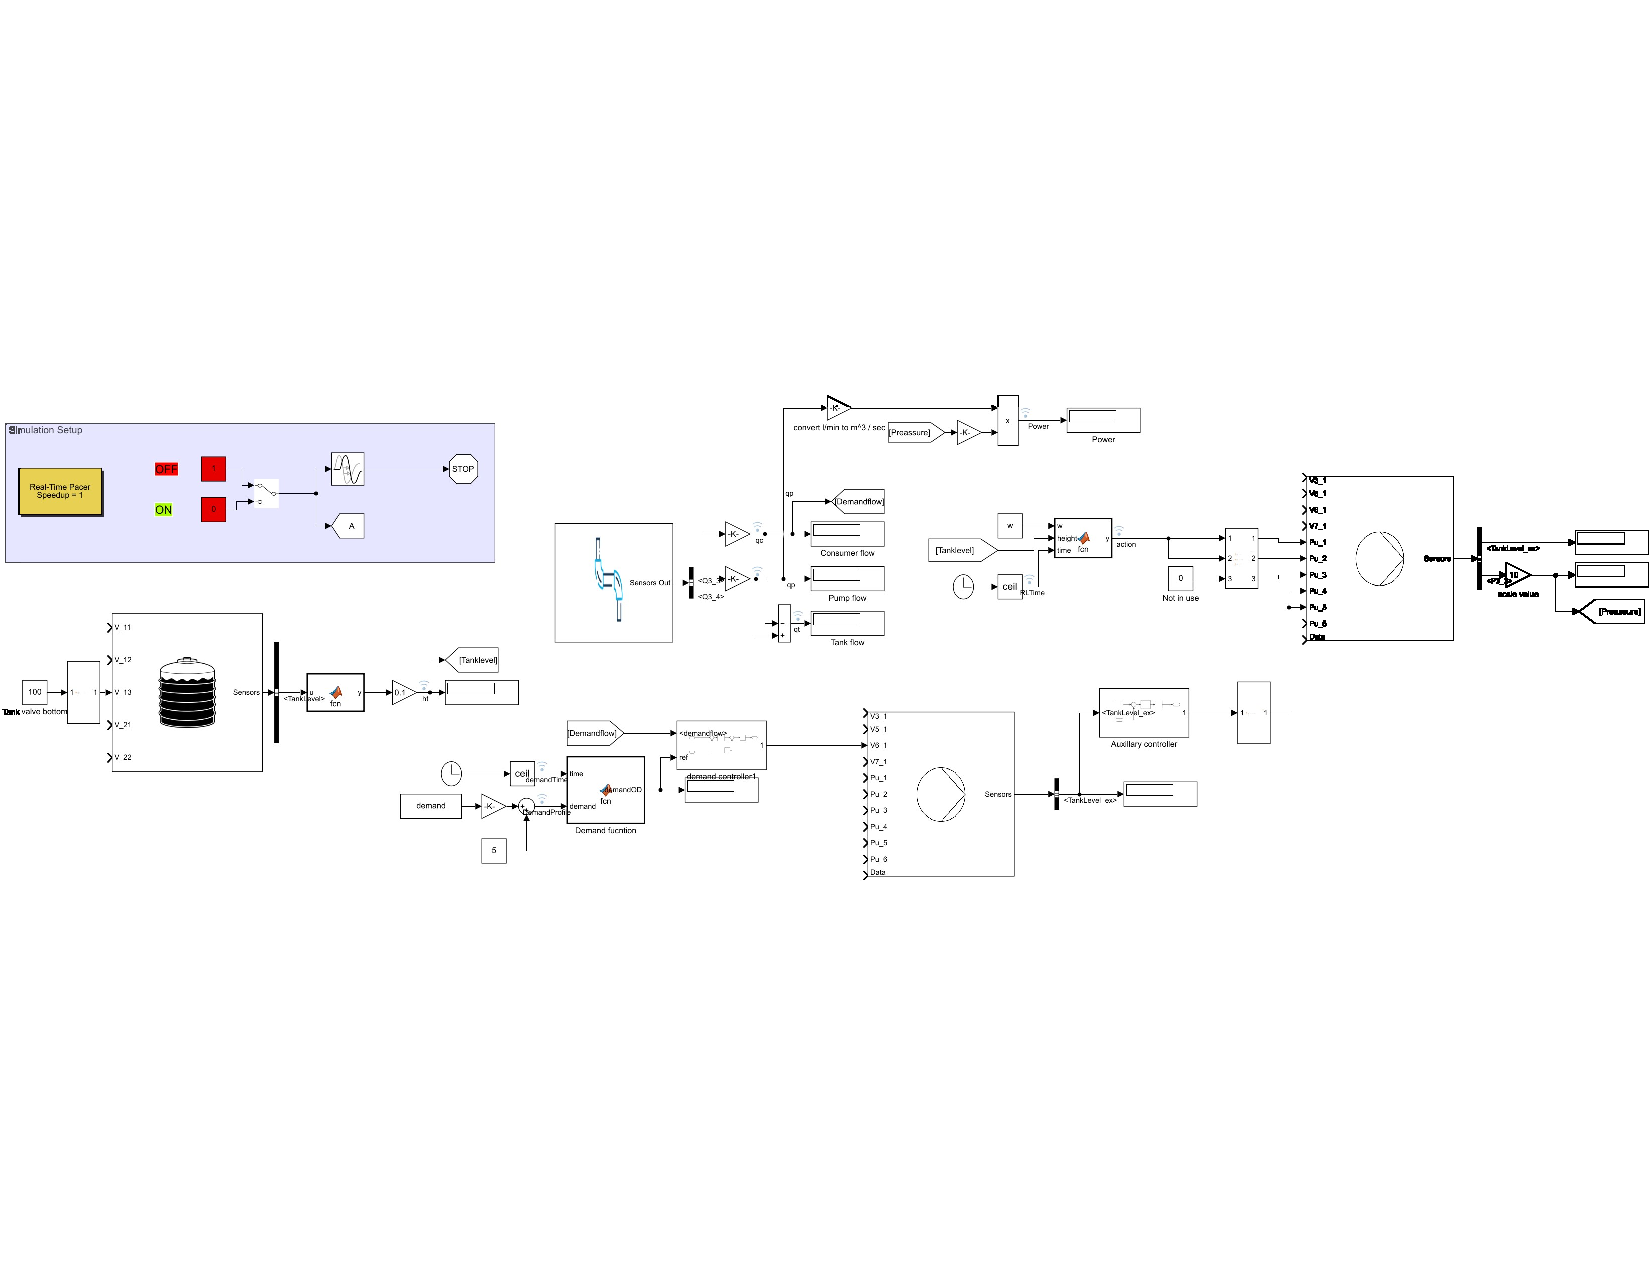
\includegraphics[width=1\linewidth]{figures/Simulink.pdf}
	\caption{Simulink setup}
	\label{fig:Simulink}
\end{figure} 
\end{document}